\appendix
% 17 Oct (v3_full): A software; B parameters and weights; C rig operations and log; D secondary results, negative
% results and history (the approaches to model error, further twin tests, wrong model values, the lever table, the 1 m
% bands, corner cutting, fault coverage, the twin's own approach, dated history one line each); E timeline; F the
% network controller of the earlier plant, condensed to dated history.

\section{Software architecture}
\label{sec:app_software}

Table~\ref{tab:app_nodes} lists the nodes of a flight and Table~\ref{tab:app_topics} the main
topics between them. The same nodes run in simulation and on the rig; only the input and output
nodes differ (the Gazebo bridges and emulators against the radio and motion-capture nodes).

\begin{table}[H]
\centering
\small
\caption{Nodes of a flight.}
\label{tab:app_nodes}
\begin{tabularx}{\textwidth}{llX}
\toprule
Package & Node & Role \\
\midrule
\texttt{mpc\_planner} & planner & Load--cable planner (10\,Hz): rod sweep, pretension, lift, trajectory, LAND; one reference per UAV \\
 & reconfiguration node & The planner in detach mode: the detection of a release, the resize for a leave and a join, the drop rule, the fold-in \\
\texttt{tracker} & \texttt{tracker\_}$i$ & Per-UAV tracking MPC (50\,Hz) with the measured rod pull; the freed UAV's landing and the take-back \\
\texttt{fleet\_manager} & \texttt{fleet\_manager} & ARM, TAKEOFF, LAND, DISARM, ESTOP; fleet-wide abort; the pre-takeoff gate \\
\texttt{drone\_communication} & \texttt{elrs\_interface} & One per UAV: CRSF frames to the radio at 100\,Hz, telemetry back, arming confirmed by the flight controller, magnet channel \\
\texttt{drone\_communication} & \texttt{motion\_capture\_publisher} & OptiTrack rigid bodies to per-body pose and velocity topics \\
\texttt{drone\_magnet} & magnet manager, \texttt{elrs\_mux} & The attach confirmation (contact and co-motion) and the radio hand-over at an attach \\
\texttt{drone\_visualisation} & panel, \texttt{fleet\_viz} & Operator panel (ARM, TAKEOFF, LAND, DISARM, magnets) and RViz scene \\
\texttt{simulation\_communication} & bridges, emulators & Gazebo only: flight controller and motion-capture emulators, clock \\
\bottomrule
\end{tabularx}
\end{table}

\begin{table}[H]
\centering
\small
\caption{Main topics.}
\label{tab:app_topics}
\begin{tabularx}{\textwidth}{lX}
\toprule
Topic & Content \\
\midrule
\texttt{/drone\_}$i$\texttt{/motion\_capture\_state}, \texttt{/payload/...} & Pose and velocity of each UAV and of the payload \\
% SETTLED 10 Oct (was a CHECK): twelve numbers per node (mpc_planner planner_node.py _publish_ref; tracker_node.py
% _planner_ref_callback): position, velocity, the planned thrust per unit mass f_i/m_q and the cable
% acceleration. The throttle feedforward is not a thirteenth number: it is the magnitude of f_i/m_q.
\texttt{/drone\_}$i$\texttt{/reference\_trajectory} & The planner's horizon for UAV $i$: node count, time step, then per node position, velocity, planned thrust per unit mass (its magnitude is the throttle feedforward, its direction the attitude reference) and planned cable acceleration (twelve numbers per node) \\
\texttt{/drone\_}$i$\texttt{/ELRSCommand} & The tracker's command: armed flag, throttle, three rate sticks, auxiliary channels \\
\texttt{/drone\_}$i$\texttt{/telemetry} & Battery voltage, flight mode, link quality \\
\texttt{/drone\_}$i$\texttt{/fc\_arm\_state} & The flight controller's own arm state and the reason for a refusal \\
\texttt{/drone\_}$i$\texttt{/magnet} & Magnet on or off \\
\texttt{/fleet/command} & ARM, TAKEOFF, LAND, DISARM, ESTOP \\
\texttt{/fleet/detach}, \texttt{/magnet/command} & DETACH of UAV $i$; ATTACH (magnet on) \\
\texttt{/fleet/abort} & Fleet-wide disarm on any fault \\
\texttt{/fleet/landed}, \texttt{/fleet/cable\_ff\_active} & Planner to fleet: landed; cable feedforward on \\
\bottomrule
\end{tabularx}
\end{table}

\section{Parameters and weights}
\label{sec:app_params}

Table~\ref{tab:app_params} sets the parameters of the rig twin against those of the rig, and
Table~\ref{tab:weights} gives the cost weights of the planner and the trackers.

\begin{table}[htbp]
\centering
\small
\caption[Parameters of the rig twin and the rig]{Parameters of the rig twin and the rig, from the launch
profiles of the final code. A value spanning both columns is flown by both; a letter marks a value that changed
during the work (notes below the table). The twin's time-outs run on simulation time.}
\label{tab:app_params}
\begin{tabularx}{\textwidth}{>{\raggedright\arraybackslash}X>{\centering\arraybackslash}p{2.9cm}>{\centering\arraybackslash}p{2.9cm}}
\toprule
Parameter & Rig twin & Rig \\
\midrule
\multicolumn{3}{l}{\textit{Fleet and payload}} \\
\quad UAV mass, with rod and magnet (kg) & \multicolumn{2}{c}{0.55} \\
\quad payload mass (kg) & \multicolumn{2}{c}{0.86} \\
\quad rod length (m) & \multicolumn{2}{c}{0.55} \\
\quad rod pivot below the UAV centre (m) & \multicolumn{2}{c}{0.04} \\
\quad attachment radius (m) & \multicolumn{2}{c}{0.225} \\
\multicolumn{3}{l}{\textit{Thrust map}} \\
\quad throttle offset $a_i$, shared & \multicolumn{2}{c}{0.185} \\
\quad voltage slope about 23.5\,V (1/V) & \multicolumn{2}{c}{0.022} \\
\quad gain above the offset, $k_T$ (m/s$^2$) & \multicolumn{2}{c}{35.2} \\
\quad throttle cap & \multicolumn{2}{c}{0.8} \\
\quad per-UAV thrust trim & \multicolumn{2}{c}{off} \\
\multicolumn{3}{l}{\textit{Takeoff and lift}} \\
\quad rod sweep (creep) speed (m/s) & \multicolumn{2}{c}{0.2} \\
\quad planned rod elevation & \multicolumn{2}{c}{60$^\circ$\,$^a$} \\
\quad hand-over: every rod within 8$^\circ$ of it for (s) & \multicolumn{2}{c}{1.0} \\
\quad pretension (s) & \multicolumn{2}{c}{3.0} \\
\quad breakaway cap on the pull & 0.75 at lift-off & at breakaway \\
\quad cap release (s) & \multicolumn{2}{c}{2.0} \\
\quad rod tautness gate, measured over typed length & \multicolumn{2}{c}{0.9} \\
\quad lift ramp (m/s) & 0.1 & 0.1\,$^b$ \\
\multicolumn{3}{l}{\textit{Height integral and tracker}} \\
\quad integral gain $k_i$ (1/s), bound (m), gate (m) & \multicolumn{2}{c}{0.4, 0.3, 0.25} \\
\quad integral conversion $K_{xy}$, $K_z$ (N/m) & \multicolumn{2}{c}{5.3, 7.1$^g$} \\
\quad tracker initial-condition box $\epsilon$ & \multicolumn{2}{c}{0\,$^c$} \\
\multicolumn{3}{l}{\textit{Landing}} \\
\quad descent speed (m/s) & \multicolumn{2}{c}{0.2} \\
\quad unwind along the rods & yes & no \\
\quad touchdown test re-armed at ring touchdown & yes & no$^f$ \\
\multicolumn{3}{l}{\textit{Reconfiguration}} \\
\quad fewest UAVs after a detach & \multicolumn{2}{c}{3} \\
\quad unannounced detach: rod over its length, 0.2\,s (m) & \multicolumn{2}{c}{0.06} \\
\quad step-out of the freed UAV (m) & \multicolumn{2}{c}{0.5} \\
\quad catch radius of the attach confirmation (mm) & [\dots] & 24 \\
\quad plate-motion condition in the confirmation & waived & yes \\
\quad drop the ring: fewer than three carriers, or ring tilt over & \multicolumn{2}{c}{30$^\circ$, every mode} \\
\multicolumn{3}{l}{\textit{Watchdogs}} \\
\quad motion-capture time-out (s) & 0.25\,$^d$ & 0.25 \\
\quad reference time-out (s) & 1.0\,$^d$ & 1.0 \\
\quad planner solve budget (s) & none & 0.06 \\
\quad flight controller confirms arming & no & yes \\
\bottomrule
\end{tabularx}

\smallskip
\parbox{\textwidth}{\footnotesize\raggedright
$^a$\,45$^\circ$ before 7 October, so the hand-over came at 37$^\circ$.
$^b$\,The rig flights of 7 and 8 October lifted at 0.15\,m/s.
$^c$\,0.025 before 4 October (Section~\ref{sec:res_ic}).
$^d$\,1.0 and 2.0\,s in the twin before 7 October.
$^f$\,After a review of its pose-freshness check.
$^g$\,Measured on the earlier stack with the planned pull.}
\end{table}

\begin{table}[h]
\centering
\caption{Cost weights.}
\label{tab:weights}
\begin{tabular}{lll}
\toprule
Level & Term & Weight \\
\midrule
Planner & payload position $(x, y, z)$ & 60, 60, 80 \\
        & payload velocity & 18, 18, 22 \\
        & attitude error, angular velocity & 5, 1 \\
        & rod direction, tension, rod rate & 25, 5, 3 \\
        & inputs $\boldsymbol{\gamma}_i$, $\eta_i$ & $10^{-3}$, $5\times10^{-3}$ \\
\midrule
Tracker & position $(x, y, z)$ & 80, 80, 40 \\
        & velocity, body rate & 2, 0.2 \\
        & stick states & $2\times10^{-4}$ \\
        & stick rates (roll, pitch, throttle, yaw) & 0.1, 0.1, 5, 0.1 \\
        & attitude error (roll, pitch, yaw) & 0.5, 0.5, 5 \\
\bottomrule
\end{tabular}
\end{table}

\section{Method details}
\label{sec:app_method}

This appendix holds the detail of Section~\ref{sec:method} that the main text summarises.

\begin{figure}[htbp]
\centering
\begin{tikzpicture}[>=Stealth, font=\small,
    blk/.style={draw, thick, rounded corners=2pt, align=center, minimum height=0.85cm, font=\small},
    ours/.style={blk, fill=blue!6, draw=blue!50!black},
    his/.style={blk, fill=orange!10, draw=orange!60!black},
    fc/.style={blk, fill=gray!12, draw=gray!60},
    lab/.style={font=\scriptsize, align=center}]
  \node[blk]  (op)   at (5.6,1.7)   {Operator\\ \scriptsize disarm button};
  \node[ours] (fm)   at (5.6,0)     {Fleet manager\\ \scriptsize phases, faults, LAND};
  \node[ours] (plan) at (0,0)       {Load--rod planner\\ \scriptsize 10\,Hz; owns the ring};
  \node[ours] (trk)  at (0,-2.5)    {Tracker $i$ (carrier)\\ \scriptsize 50\,Hz; owns UAV $i$};
  \node[ours] (trkn) at (5.6,-2.5)  {Tracker (newcomer)\\ \scriptsize from the attach, or take-back};
  \node[his]  (tej)  at (11.3,-2.5) {Collaborator's controller\\ \scriptsize pickup, transit, drop,\\ \scriptsize descent to contact, lift};
  \node[ours] (mux)  at (5.6,-4.6)  {Mux\\ \scriptsize one owner, latched};
  \node[fc]   (bf)   at (0,-4.6)    {Flight controller $i$\\ \scriptsize Betaflight rate loop, magnet};
  \node[fc]   (bfn)  at (5.6,-6.3)  {Flight controller (newcomer)\\ \scriptsize Betaflight rate loop, magnet};
  \draw[->, thick] (op) -- node[lab, right] {commands} (fm);
  \draw[->, thick] (fm) -- node[lab, above] {phase} (plan);
  \draw[->, thick] (plan) -- node[lab, left] {reference,\\ rod pull} (trk);
  \draw[->, thick] (plan.south east) -- node[lab, sloped, above, pos=0.55] {once folded in} (trkn.north west);
  \draw[->, thick] (trk) -- node[lab, left] {throttle, rates,\\ arm, magnet} (bf);
  \draw[->, thick] (trkn) -- (mux);
  \draw[->, thick] (tej.south) -- ++(0,-1.25) -- node[lab, above] {until the attach} (mux.east);
  \draw[->, thick] (mux) -- node[lab, right] {one command stream} (bfn);
  \draw[->, thick, dashed] (trk) -- node[lab, above] {fault} (trkn);
  \draw[->, thick, dashed] (fm) -- node[lab, right] {LAND, drop, disarm} (trkn);
  \draw[->, thick, dashed] (fm.north west) -- ++(0,0.5) -| node[lab, pos=0.25, above] {arm, disarm, LAND} ([xshift=-0.5cm]plan.north west) |- (trk.west);
  \draw[<->, thick, dotted] (fm.east) -| node[lab, pos=0.25, above] {attach confirmed, give-up} (tej.north);
\end{tikzpicture}
\caption[The cascade and its owners]{The cascade and its owners. Blue: this work; orange: the collaborator's
controller; grey: the unmodified flight controllers. The planner owns the ring and the carriers' references; each
tracker owns one UAV's radio link; the newcomer's link is owned by the collaborator's controller until the attach
is confirmed and by this work's tracker from that tick, through a multiplexer that latches. Dashed: faults and the
fleet manager's commands; dotted: the confirmation and the give-up exchanged with the collaborator's stack. The
operator's disarm overrides everything.}
\label{fig:owners}
\end{figure}

\subsection{The tracker's problem and the model integral in detail}
\label{sec:app_integral}

The tracker solves, every 20\,ms,
\begin{equation}
\begin{aligned}
    \min \quad & \sum_{k=0}^{N_h-1} \big\| \mathbf{h}(\mathbf{x}_k, \mathbf{u}_k) - \mathbf{h}_k^{\mathrm{ref}} \big\|_{Q}^{2} + \big\| \mathbf{h}_{N_h}(\mathbf{x}_{N_h}) - \mathbf{h}_{N_h}^{\mathrm{ref}} \big\|_{Q_{N_h}}^{2} \\
    \text{s.t.} \quad & \mathbf{x}_{k+1} = \mathbf{F}_i(\mathbf{x}_k, \mathbf{u}_k; \mathbf{a}_{c,i,k}), \qquad \mathbf{x}_0 = \hat{\mathbf{x}}_i(t), \\
    & 0.05 \le u_{T,k} \le u_{T,\max}, \quad |c_{\phi,k}|, |c_{\theta,k}|, |c_{\psi,k}| \le 1, \quad |\mathbf{u}_k| \le \overline{\mathbf{u}},
\end{aligned}
\label{eq:trk_ocp}
\end{equation}
with $\mathbf{h} = [\mathbf{p}, \mathbf{v}, \boldsymbol{\omega}, \mathbf{c}, \mathbf{u}, \mathbf{e}_R]$, the
attitude reference being the direction of the planned thrust \eqref{eq:thrust_req}. The stick states
are normalised to $[-1, 1]$, and $\overline{\mathbf{u}}$ limits how fast each may change (throttle
0.5\,s$^{-1}$). Only the first command of each solution is sent.




\paragraph{Properties.} At an equilibrium with the gate open ($G = I$) and no component of $\mathbf{b}$
saturated, $\mathbf{b}_{k+1} = \mathbf{b}_k$ gives $\mathbf{e} = \mathbf{0}$, whatever the constant cause:
by the internal model principle \cite{francis1976internal}, the integrator is the model of a constant.
This assumes stability; it does not give it. Approximating the cascade's response to $\mathbf{d}$ by a
first-order lag with time constant $\tau$, each axis becomes
\begin{equation}
    \tau s^2 + s + k_i = 0, \qquad \zeta = \frac{1}{2\sqrt{k_i \tau}},
\end{equation}
so a faster integral costs damping, and delays through the planner and the radio link reduce the margin
further. Let an unmodelled constant force
$\mathbf{F}$ act on the payload and let the cascade, of actual stiffness $K_c$, be quasi-static (fast
compared with the integral). The plan cancels the force it believes in, so the payload settles at
$\mathbf{e} = -K_c^{-1}(\mathbf{F} - \mathbf{d}) = -K_c^{-1}(\mathbf{F} + K\mathbf{b})$, and in continuous time
\begin{equation}
    \dot{\mathbf{b}} = k_i\,\mathbf{e} = -k_i K_c^{-1}\big(K\mathbf{b} + \mathbf{F}\big)
    \quad\Rightarrow\quad \mathbf{b} \to -K^{-1}\mathbf{F}, \qquad \mathbf{d} \to \mathbf{F},
\end{equation}
a first-order convergence at the rate $k_i K K_c^{-1}$ on each axis, with time constant $1/k_i = 2.5$\,s when
$K = K_c$. The believed force converges to the applied one whatever $K$ is: $K$ sets only the speed, and
too large a $K$ costs damping as too large a $k_i$ does. When the force is removed, $\mathbf{b}$ still holds
$-K^{-1}\mathbf{F}$, so the payload overshoots by $K_c^{-1}\mathbf{F}$, the displacement the force caused at
onset, and the overshoot decays at the same rate. This analysis assumes that the force reaches the payload's
position error. With the measured rod pull (Section~\ref{sec:tracker}) a constant vertical force is taken up at
each UAV within about a second, before the integral can act, so in the twin the integral is left with the
horizontal axes (Section~\ref{sec:res_force}).

\paragraph{Reference-shift form.} An earlier version added the height integral to the payload's height
target instead, $z_L^{\mathrm{ref}} \leftarrow z_L^{\mathrm{ref}} + b_z$. Both forms reach the same steady
state; in offset-free MPC they are output and input disturbance models, which differ in the transient, not
in the steady state \cite{pannocchia2007combined}. The model form keeps the target fixed, so its plan
predicts a payload held at the target, which is what happens; the reference-shift form plans a move towards
a shifted target that never comes. The model form also extends to the horizontal axes, and it is the
default everywhere, a resizing fleet included (the integral's force is kept through the resize). The
reference-shift form, on the height only, flies where the model form cannot, and flew on the rig on 1 and
8 October ($k_i = 0.4$\,s$^{-1}$); the 7 October carry flights flew the model form.
% Model integral through a resize since 8 Oct (896aff2; bringup real_mode.planner_options).
% STATUS 5 Oct 2026: int_mode auto (model where allowed, else reference): reference with kt_trim on,
% a resizing fleet, z_ki 0, offset_free on or dist_est ring/full (bringup real_mode.planner_options).

\paragraph{Bound and limits.} $\bar{b} = 0.3$\,m bounds the force the integral can supply to $K\bar{b}$
(2.1\,N vertically), enough for an unmodelled 0.1\,kg object. A larger error is a fault, not a disturbance,
and a warning at 70\,\% of the bound reports it rather than covering it silently; the bound and the warning are
also what stop an integral that winds up without effect, as the vertical integral does on a wrong attachment
radius in the twin (Section~\ref{sec:sim_robustness}). A force on the payload cannot represent a moment: one UAV's
thrust-map error is a moment on the ring, which that UAV's own tracker takes up through its measured pull. A miss
larger than the gate is never integrated. The integral is also slow ($1/k_i = 2.5$\,s): it removes constant and
slowly varying forces, not impacts or gusts. Five other ways to remove a steady error were built and flown on the
earlier stack (a force balance \cite{muske2002disturbance}, an offset-free observer
\cite{pannocchia2003disturbance}, the measured cable force, a per-UAV thrust-gain trim, and the rods' mass in the
planner); Appendix~\ref{sec:app_methods} records them, and the measured cable force became the trackers' measured
pull.

\subsection{Reconfiguration: the ramp, the seed, the fall-backs and the constants}
\label{sec:app_reconfig}

\paragraph{The ramp and the seed.} Where the planner is told of a change it can shape the step. For a ramped
release the leaver's planned tension is run down and the survivors' run up over a short ramp before the magnet is
released, in place of a step at the resize tick; the first version of the ramp, which ran the leaver's tension
down but let the survivors' step, is the negative that defined it. For a join the newcomer is seeded at 0.1\,N and
every tension is blended to the balanced solution for the new geometry, as a dock blends thrust across its
controller switch \cite{sugihara2023trady}: on the earlier plant a newcomer started at a full share pulled the ring
with a lever about the incumbents' rod apex and tilted it at the weld (Appendix~\ref{sec:app_proximity_weld}).



\paragraph{The freed UAV.} After a release the freed UAV steps 0.5\,m out radially at its height, clear of the ring
and the survivors, and lands by itself while the survivors carry on: its height reference is pressed below its own
resting height until it is there, and it is then disarmed alone, without waiting for the fleet
(Section~\ref{sec:res_freed}). Touchdown for the fleet is judged on the survivors only, so a freed UAV still
descending elsewhere does not hold their references down, and the fleet is declared landed only when it is down
too; the rod feedforward is switched off once the ring rests, because its sideways component pushes a grounded
survivor across the floor.

\paragraph{The take-back.} A newcomer whose contact is not confirmed within its timeout, or whose controller gives
up, is taken back: this work's tracker latches onto its measured position and velocity, ramps its reference at
0.25\,m/s$^2$ so that the latch makes no step, lifts it clear of the rim and the carriers, moves it out and lands it
by itself. On the circle the hold moves with the ring in the ring's planned frame, so that an orbiting formation
cannot sweep a carrier into the newcomer's rod; where the newcomer is low and far out, it lands where it stops. On
the rig the take-back first rises only 5\,cm above the tether's slack and waits for the tip to leave the plate, so
that a magnet that has caught after all is not torn off; if the plate rises instead, the magnet is switched off
again and the fleet lands. The tilt cut, the drop rule and LAND are the exits of Section~\ref{sec:safety}.

\paragraph{The rejoin mission.} The full mission is assembled with the collaborator's mission planner. Four UAVs
carry the ring in hover or round the circle; the one on plate 9 is released and flies the collaborator's errand
(picking up an object with its magnet and dropping it into the ring) and comes back to its plate; it is admitted
under the contract above, folded in, and the fleet lands. On the rig the collaborator's controller does every
attach down to contact, since the magnet catches only on the plate; this work's own approach, which steered the
measured magnet tip and welded on proximity, flies in the twin only (Appendix~\ref{sec:app_proximity_weld}).


\begin{table}[htbp]
\centering
\small
\caption[Reconfiguration constants and their reasons]{The constants of the reconfiguration and the reason for each
value: a noise floor times a factor, or a physical bound. [Bracketed reasons wait for the offline sweeps over the rig
recordings.]}
\label{tab:constants}
\begin{tabularx}{\textwidth}{>{\raggedright\arraybackslash}p{3.6cm}>{\raggedright\arraybackslash}p{2.4cm}>{\raggedright\arraybackslash}X}
\toprule
Constant & Value & Reason \\
\midrule
Rod stretch for an unannounced leave & 0.06\,m, two ticks & A rod on its plate cannot read longer than itself; the
threshold sits above the scatter of a rod length measured from motion capture, and two ticks reject a single bad
pose. [False alarms over the rig recordings and delay against threshold from the rig releases.] \\
Contact & catch radius 24\,mm (rig); face $-15$ to $+12$\,mm; under 0.03\,m/s for 0.3\,s & The magnet catches only on
the plate: the tip must be over the plate's face and at it, and still for 36 motion-capture samples, which excludes a
pass over the plate. \\
Confirmation, 1.0\,s after the lift & tip within 6\,mm of its contact point; plate range 5\,mm or rise 3\,mm; taut
within 3\,mm & A caught tip moves with the plate and a missed one is left behind by it; the free hang is measured on
each flight, so the taut check reads this flight's tether. \\
Confirmation fails & 45\,mm for 0.12\,s; any data gap over 0.1\,s restarts & A tip that leaves the plate has not
caught; no hold is judged across missing poses. \\
Newcomer's seed tension & 0.1\,N & Small against the newcomer's balanced share (1.6\,N on plate 9 of the carry
layout), so the fold-in's blend and not the weld sets the step. \\
Step-out after a release & 0.5\,m radially & Clears the rim (0.255\,m) and the survivors' rods from the leaver's
plate. \\
Take-back ramp & 0.25\,m/s$^2$ & A quasi-static tilt of 1.5$^\circ$ on the newcomer, under the 2$^\circ$ bar on its
attitude step, and it stops 0.34\,m/s in 1.4\,s. \\
Take-back clearances & 0.15\,m over the carriers; 0.3\,m under the ring; 0.9\,m from the ring's centre & The
newcomer's body and rod stay a rotor disc clear of the carriers; a low newcomer lands where it is rather than
rising through the formation. \\
Ring tilt that drops the ring & 30$^\circ$ & Beyond the planner's near-level model and about where a rod's pull turns
across its plate; where the controller gives up, not a value to design to (Section~\ref{sec:safety}). \\
Fewest carriers & 3 & Two rim points make the ring a pendulum about the line between them. \\
\bottomrule
\end{tabularx}
\end{table}

\subsection{Metrics in full}
\label{sec:app_metrics}

\begin{description}
\item[Release metrics] For a UAV leaving the team, frozen on 11 October before the first flight they
    score; one rule for the twin and the rig. The ring's tilt is kept as a vector: with $\mathbf{n}$ the ring's
    body $z$ axis in the world frame, the tilt angle is $\arctan\!\big(\sqrt{n_x^2+n_y^2}\,/\,n_z\big)$ and
    the tilt vector $\boldsymbol{\theta}$ is that angle along the horizontal direction of $\mathbf{n}$, so that
    $|\boldsymbol{\theta}|$ is the scalar tilt above. The event time $t_e$ is the DETACH command for an announced
    release, the magnet's OFF for an unannounced one (the runner's RELEASE in the twin, the first magnet OFF in
    the rig's bag), and the first planner tick at which the leaver's planned tension falls for a ramped release;
    LAND is the LAND command. Over the pre-window $[t_e-5\,\mathrm{s},\,t_e)$ the mean
    $\bar{\boldsymbol{\theta}}_{\mathrm{pre}}$ and the spread
    $\sigma_{\mathrm{pre}}=\sqrt{\overline{|\boldsymbol{\theta}-\bar{\boldsymbol{\theta}}_{\mathrm{pre}}|^2}}$
    are taken. A row whose ring reference was not still for the 5\,s before the event (its height within
    5\,mm of its value at $t_e$ and its speed within 0.02\,m/s of its median over the last 2\,s) is flagged and
    still reported. \textbf{Tilt rise} $\Delta\theta$, the primary metric, is the maximum of
    $|\boldsymbol{\theta}(t)-\bar{\boldsymbol{\theta}}_{\mathrm{pre}}|$ over $[t_e,\,\mathrm{LAND}]$; when two
    runs are compared both are cut at the shorter hold, each 8 October pair at the rig flight's event-to-LAND,
    and the ledger's bands and the flights they score at $t_e+15$\,s. Beside it: the absolute peak,
    $\max|\boldsymbol{\theta}|$ over the same window, and the scalar rise, the absolute peak minus the mean of
    $|\boldsymbol{\theta}|$ over the pre-window. The 30$^\circ$ drop rule and the join bars stay on the
    absolute tilt. \textbf{Time back in band:} with $\bar{\boldsymbol{\theta}}_{\mathrm{post}}$ the mean over
    the last 5\,s before LAND, scored only when LAND comes at least 10\,s after $t_e$, and the half-width
    $b=\max(2\sigma_{\mathrm{pre}},\,0.5^\circ)$, it is the earliest $t$ at or after the time of $\Delta\theta$
    such that $|\boldsymbol{\theta}-\bar{\boldsymbol{\theta}}_{\mathrm{post}}|\le b$ for every sample in
    $[t,\,t+1\,\mathrm{s}]$, reported as $t-t_e$, or ``not back''. The dip (the largest drop of the ring's
    height below its pre-event mean), the detection time (from the magnet's OFF to the planner's resize), the
    steady offset, the landing lean, the clearances and the survivors' shares keep their scorers and are not
    part of the freeze.
    \item[Join metrics] For a newcomer admitted to the ring: the time from the last contact to the confirmation; the ring's
    tilt rise, on the release metric above with the contact as the event, from the contact to 8\,s after the
    confirmation; the ring dip over the same window; the hand-over step, the change in the newcomer's applied
    throttle, roll, pitch and yaw-rate commands between the 0.1\,s before the switch of authority and the 0.3\,s
    after it, as a fraction of its hover throttle and in degrees; the newcomer's tilt at the confirmation; and the
    clearances of the newcomer's body and rod to every carrier body and rod through its approach and, when it is
    taken back, through its take-back. For the full mission, also the tilt at the release, the mean tilt over the
    circle and the time from TAKEOFF to every UAV landed.
    \item[Magnet margin] For a release, the survivors' peak measured rod pull and the rate at which it rises,
    against the magnet's hold at that rod angle (Section~\ref{sec:hardware}); the one metric that says how close a
    transient came to letting a second magnet go.
    \item[Switch validation] For every resize, the planner's solver status and residual at the first live solve
    after the switch, the distance of that solve from an offline solve of the same logged problem run to
    convergence (not computed so far: the planner keeps a problem only when its solve fails), the solve time against the 60\,ms budget on the rig, and the step in each survivor's commanded
    throttle across the switch.
    \item[Solver health] The number of planner solves that failed or did not converge.
\end{description}

Every arm of a lever table and every ledger row is labelled a \emph{replication} when both arms of a twin pair, or the
rig flight of a ledger row, were flown and registered before the rule was signed on 11 October, and a \emph{new
prediction} otherwise; the label is set at the signature and never changes.

\paragraph{Why these bars.} Three physical limits say what a transient may do to the ring, and the bars of the
results sections sit inside them. The first is the magnets. A plate holds its magnet straight off the face by
about 9--10\,N and by less under shear, so a tilt that turns a rod's pull across its plate can let a magnet go:
every ring lost on the rig began with a magnet letting go with no command, two with the rods planned at
45$^\circ$ and two since the rods have been planned at 60$^\circ$ to keep each pull closer to its plate's axis
(Section~\ref{sec:res_leave}). [The hold against the angle of pull, still to be measured with a spring scale,
gives this limit its number.] The second is the fleet's own rule:
a ring tilt over 30$^\circ$, or a loss that leaves fewer than three carriers, drops the ring and lands every UAV
(Section~\ref{sec:safety}), so
30$^\circ$ is where the controller gives up, not a value to design to. The third is the model: the planner's
load--rod model and each tracker's rod pull assume a near-level ring, so a transient that stays within a few
degrees stays inside the regime the plan was computed for, and a transient that leaves it is being flown on a
plan that no longer describes the ring. The bars are therefore stated as a rise above the ring's own motion
before the event, small against the first two limits and inside the third, and every run is reported with its
measured rise so that a run that misses a bar is still read against the limits rather than against a number.


\section{Rig operations and log}
\label{sec:app_rig}

\subsection{Arming, preflight checks and flight procedure}

\paragraph{Arming.} Betaflight refuses to arm while any of its arming checks fails, and then waits
for the arm switch to go low and high again. A switch raised at such a moment is ignored until it is
toggled, which is the likely reason two of the UAVs often failed to arm on the first attempt on the
rig and armed after a power cycle. Each UAV's radio node therefore holds the arm switch low for
0.3\,s before raising it, confirms the arm from the flight mode the flight controller reports, and
retries with a fresh switch edge up to three times. This has been tested against a simulated flight
controller, not yet on the rig. The fleet manager waits
for every flight controller to report armed and names any UAV that did not, with the reason it
reported, before TAKEOFF is accepted.

\paragraph{Preflight checks.} Before each flight a script checks, from the live topics:
motion capture for every UAV and the payload (fresh, above 20\,Hz, no missing values); each UAV
resting level (under 20$^\circ$) and the payload resting level (under 25$^\circ$); every battery
above 23.6\,V and its telemetry present; the same magnet channel on every radio; the parameters the
controllers actually loaded (masses, rod length, attachment radius, thrust map, throttle cap);
each UAV within tolerance of its typed attachment azimuth; and each rod length from motion capture.
It reports GO or NO-GO.

\paragraph{Flight procedure.} Each flight is started with one command that clears leftover
processes, records every relevant topic and writes the logs to a per-flight folder, so that every
flight can be read back before the next. The operator holds a disarm button on the ground station;
a disarm or a fault on any UAV disarms the whole fleet.

\paragraph{Test ladder.} New behaviour is flown in an order that isolates one effect at a time:
free hover, to check the thrust map; then the payload held at its lift height; hover; the circle and
the figure-8; the detach; and the attach last. Each step is first flown in the rig twin with the
same launch commands.
% Moved 9 Oct (page trim) from the method's experimental process (Section 3.9.1).

\subsection{Floor start and landing in detail}
\label{sec:app_floor}

\paragraph{Why the planner cannot start from the floor.} With the payload resting and the rods flat,
the UAVs sit about 0.7\,m from the payload's centre, 18--22\,cm outside the 45$^\circ$ cone on which the
planner's references put them. Started from rest, the planner pulled the UAVs inwards over the payload
instead of lifting it, the cause of the first failed lifts on the rig.

\paragraph{Rod sweep (creep).} On TAKEOFF each UAV is anchored where it rests, and its rod is swept about
its own attachment point at a constant rate, from its measured elevation to the planned elevation, 45$^\circ$
until 7 October and 60$^\circ$ since. The UAV's reference is the far end of the rod on that arc, so the rod stays
straight and the UAV never moves over the payload. The planner takes over (the hand-over) once every rod has
been within 8$^\circ$ of the planned elevation for 1\,s (at least 37$^\circ$ before 7 October), or 3\,s after
the sweep ends. The hand-over is refused below 30$^\circ$, because from
shallower rods the lift needs two to three times the tension, mostly sideways.

\paragraph{Rod lengths.} At the hand-over the planner measures each rod from motion capture, from the
UAV's pivot to its attachment point, and uses the measured lengths in its model and its tautness gate.
A measurement is accepted if each rod is within 25\,\% of the typed length and the rods agree within
8\,cm; otherwise the typed length is kept and the reason logged. Without this, a rod shorter than typed
reads as partly slack to the gate (Section~\ref{sec:sim_robustness}).
% --- original text, flown before the rig twin; kept to refill this place:
% Without this, a rod 4\,cm shorter than typed reads as slack to the gate and the fleet flies only
% part of the cable feedforward (Section~\ref{sec:sim_robustness}).

\paragraph{Pretension.} The rods are then loaded before the payload leaves the floor: every UAV's share
of the cable feedforward rises together from zero to its planned value over 3\,s, with the height target
at the resting height. A step in the planned pull here launched the payload and released two magnets on
the rig, and UAVs pulling one after another tilted it.

\paragraph{Breakaway.} When the payload rises 1\,cm, or its vertical speed exceeds 0.03\,m/s, it has broken
free of the floor, and the fraction of the planned pull reached at that moment is frozen as a cap on the
feedforward; continuing the ramp with the payload in the air ran it upwards at 0.38\,m/s on the rig. Once
the lift starts, the cap is released back to full pull over 2\,s. Holding it for the whole flight, as in
the first rig flights, leaves the trackers believing the rods pull less than they do, and the payload
settles low (Section~\ref{sec:res_cap}).

\paragraph{Lift.} The height target then ramps from the resting height to the target height at 0.1\,m/s,
easing in over the first 1.2\,s and out over the last 8\,cm, and the trajectory starts when the ramp
completes.

\paragraph{Landing.} On LAND the planner lowers the payload's height target at 0.2\,m/s, with the formation
shape unchanged, until the payload rests on the floor. A rigid rod then constrains its UAV: a UAV
descending straight down is pushed outward as its rod lengthens horizontally, by 16--20\,cm in the rig
twin, and this tipped UAVs over in a few landings. Three measures remove this.
\begin{itemize}
    \item \textbf{Unwind.} Each UAV's reference moves out along its rod's circle about the grounded
    attachment point, at the landing speed, down to level, and then straight down. Below 0.25\,m the
    horizontal reference follows the UAV. Twin only: the rig's slack tethers let it land straight down.
    \item \textbf{Feedforward ramp.} The planner blends each UAV's thrust and cable feedforward to plain
    hover over 1\,s, instead of dropping the cable term in one step at touchdown, which left the attitude
    oscillating while the rods still acted.
    \item \textbf{Ground idle.} A UAV that has flown and is back within 3\,cm of its resting height, with
    the payload down and its reference at the floor, switches to armed idle until the fleet disarms;
    otherwise a UAV that lands first tracks a reference below the floor and rocks on its feet.
\end{itemize}
Touchdown is detected when the UAVs stop following the descending reference for 1\,s, after descending at
least 5\,cm; the planner then reports the fleet landed and the fleet manager disarms it. In the twin the test is
re-armed when the ring touches down (Section~\ref{sec:sim_landing}), and it reads only poses fresher than 0.2\,s,
so that a frozen pose cannot read as a stall.

\subsection{Rig days}

The rig is available about two days a week, and each day followed the simulation work of the days
before it, so each is summarised with what it showed and what changed as a result
(Table~\ref{tab:rig_days}).

\begin{table}[h]
\centering
\small
\caption{Rig sessions with the payload, to 15 October.}
\label{tab:rig_days}
\begin{tabularx}{\textwidth}{lX}
\toprule
Date & What was flown and what it showed \\
\midrule
3 Aug & First flights of the planner stack on the rig. Fixed: attachment slots matched in the
payload's frame (a yawed payload made the problem infeasible), a latched payload yaw datum, a latched
heading per UAV (one UAV turned a full circle on takeoff), trackers on the correct clock. \\
16 Sep & First carry attempts with the planner from the floor: the payload did not lift. One UAV per
flight spun in yaw at spool-up, later traced to the tracker's yaw command on a tilted floor rest. The planner's references assumed taut rods and sat inside
the UAVs (Section~\ref{sec:takeoff}). \\
23 Sep & Two UAVs, rods typed 0.50\,m against a real 0.46\,m, thrust gain typed: the payload did not
leave the floor and the UAVs drifted in over it. One battery sagged from 21.2 to 17\,V. Found: battery
thresholds set for a smaller battery, and the need for the rod sweep. \\
30 Sep & Four UAVs, 0.86\,kg ring. First lifts and the first sustained carry (12.6\,s at 0.28\,m). Seven
bugs fixed on the day. The thrust map identified (Section~\ref{sec:thrust_id}). Breakaway at 60--80\,\%
of the planned pull. Last flight: ring held 16\,cm low with a 14\,cm heave at 0.17\,Hz, and 25 planner
solve failures. \\
1 Oct & Three UAVs (one airframe out of service), six flights to 1.0\,m including a circle and a
figure-eight, with no solve failures (Table~\ref{tab:rig_oct1}). \\
7 Oct & Four UAVs: the cap release, the pinned initial condition and the model integral in hover
(Figure~\ref{fig:rig_integral}); the circle and the figure-eight on the planner's and then the measured pull with
the rods planned at 60$^\circ$ (Table~\ref{tab:T7}); two announced releases, one carried through and one lost when two
magnets let go; on the even ring a magnet let go in the circle (Table~\ref{tab:T8a}). \\
8 Oct & Four releases of one UAV of four on the measured pull, announced and unannounced, in hover and on the
circle, all carried through; the body rates sent at full precision from the evening. \\
14 Oct & 46 launches with the collaborator's controller and the combined stack: the first attach flights, with one
contact rejected by the proof of the day; a three-carrier lift that lost the ring when a carrier's magnet let go
(L10); arm refusals from two flight controllers' attitude drift; the drop rule turned on in every mode, and the
co-motion confirmation written that evening. \\
15 Oct & Attach flights on the co-motion confirmation, no contact; a carrier's magnet let go in hover and the drop
rule landed the fleet (L11); a LAND in the collaborator's match phase ended in a take-back; the lab asked for flights
of four UAVs at once to stop until a noise approval. \\
\bottomrule
\end{tabularx}
\end{table}

\begin{table}[h]
\centering
\small
\caption{Rig flights on 1 October, three UAVs on plates 0, 4 and 8. Breakaway: fraction of the planned
pull at which the ring left the floor; it was held for the whole flight. Height integral bound
0.15\,m. Tilt and the horizontal offset are over the hold; $^{\dagger}$ marks the mean distance from
the trajectory reference over the manoeuvre. Orbit: radius 0.5\,m at 0.125\,m/s; figure-eight:
$a = 0.5$\,m at 0.2\,m/s. Rotated: the whole system turned by 124$^\circ$; moved: shifted 1.1\,m
towards $+x$.}
\label{tab:rig_oct1}
\footnotesize
\begin{tabularx}{\textwidth}{>{\raggedright\arraybackslash}Xcccccc}
\toprule
Flight & Target & Held & Integral & Tilt & Offset & Break- \\
 & (m) & (m) & & mean / max & (cm) & away \\
\midrule
Hover & 0.5 & 0.45 & off & 5.0 / 13.8$^\circ$ & 5.7 & 80\,\% \\
Hover & 0.8 & 0.67 & at bound & 2.5 / 6.7$^\circ$ & 11.8 & 73\,\% \\
Orbit & 1.0 & 0.94 & at bound & 1.6 / 4.1$^\circ$ & 15.1$^{\dagger}$ & 83\,\% \\
Figure-eight & 1.0 & 0.67 & never on & 3.2 / 9.0$^\circ$ & 18.8$^{\dagger}$ & 73\,\% \\
Hover, rotated & 1.0 & 1.01 & at bound & 3.8 / 6.6$^\circ$ & 8.1 & 93\,\% \\
Hover, moved & 1.0 & 0.89 & at bound & 2.2 / 4.1$^\circ$ & 3--5 & 77\,\% \\
\bottomrule
\end{tabularx}
\end{table}

\paragraph{30 September.} The day went from a ring that would not leave the floor to sustained
carries. The bugs found on the day each had a clear signature in the logs. The creep fed the UAVs to the
wrong plates, so the fleet flew into the middle of the ring. The cable feedforward was zeroed while the
ring rested, so the lift deadlocked. Only one UAV received the pull flag. The pull arrived as a step
and launched the ring, releasing two magnets. Each was fixed and then flown, which is how the
pretension and breakaway procedure of Section~\ref{sec:takeoff} came about. Two problems remained at
the end of the day: the ring was held low (Section~\ref{sec:res_cap}), and the planner failed to solve 25 times in the last
flight.
A replay of the planner on the logged states traced the failures to two faults acting
together. The UAVs sat 30$^\circ$ round from the attachment points the planner modelled, one plate off,
and the payload's measured quaternion changed sign when its yaw crossed 180$^\circ$. Removing either
removed every failure in the replay. The planner now keeps the quaternion's sign continuous and
warns before ARM if a UAV sits more than 10$^\circ$ from its slot. None of the 1 October flights had a
solve failure.

\section{Secondary figures and results}
\label{sec:app_secondary}

The figures and analyses that support Section~\ref{sec:results} but that its claims do not need on the page.

\subsection{Carrying}

\begin{table}[htbp]
\centering
\footnotesize
\setlength{\tabcolsep}{2.6pt}
\caption[The carry in the twin on 1\,m cables]{The carry arm with 1\,m cables, as Table~\ref{tab:T7t}: two runs per
cell, the range over the two runs.}
\label{tab:T7t1m}
\begin{tabular}{llccccccc}
\toprule
 & & \multicolumn{2}{c}{Scored} & \multicolumn{5}{c}{Reported} \\
\cmidrule(lr){3-4}\cmidrule(lr){5-9}
 & Speed & Ring RMSE & Peak tilt & Path RMSE & Path tilt & Cut & Across rms & Lag \\
Path & (m/s) & (mm) & ($^\circ$) & (mm) & ($^\circ$) & (mm) & (mm) & (ms) \\
\midrule
Circle & 0.125 & 10.3--11.1 & 1.8 & 4.8--5.8 & 0.9--1.0 & 2.3--3.3 & 2.9--3.9 & 63--82 \\
Circle & 0.2 & 12.1--12.4 & 1.8--2.0 & 9.3--9.4 & 1.4--1.7 & 6.8--7.7 & 9.4--9.6 & 72--77 \\
Figure-eight & 0.2 & 14.6--16.0 & 1.7--2.5 & 14.3--15.7 & 1.7--2.3 & 20.4--20.6 & 13.1--14.7 & 36--56 \\
Line & 0.2 & 11.0--12.0 & 1.9--3.0 & 9.6--11.2 & 1.6--3.0 & -- & 1.2 & -- \\
Orbit & 0.2 & 11.9--13.2 & 2.2--2.8 & 11.5--12.6 & 1.8 & 8.2--9.5 & 8.4--9.8 & 48--60 \\
\bottomrule
\end{tabular}
\end{table}

\begin{figure}[h]
\centering
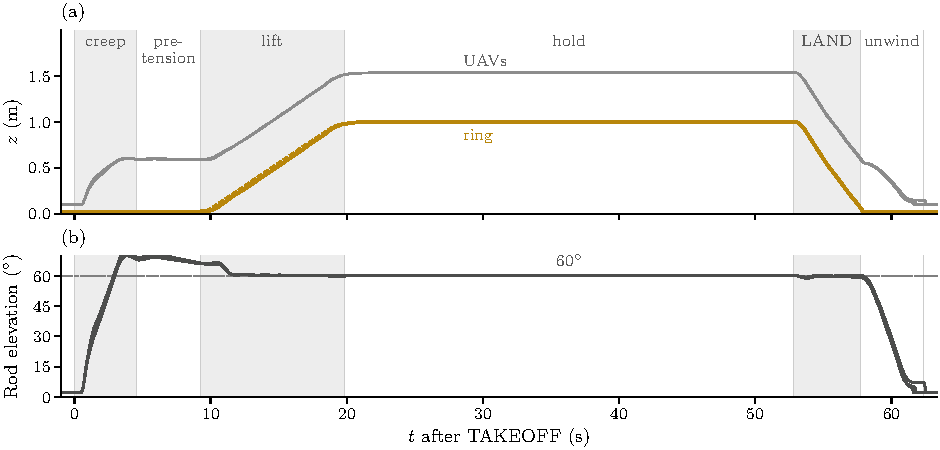
\includegraphics[width=\textwidth]{Images/flight.pdf}
\caption[One flight from the floor]{One flight from the floor in the rig twin: three carriers, hover at 1.0\,m, the
default controller (their traces overlap). (a) Heights of the ring (gold; dashed: its planned height) and of the
UAVs (grey); shaded: the creep, the lift and LAND. (b) Elevation of each rod above the horizontal; dotted: the
planned 60$^\circ$. In the creep the UAVs climb and swing their rods up from the floor, past the planned elevation,
without lifting the ring; in the pretension they hold their height while the rod feedforward eases in; the ring
then leaves the floor and follows its lift ramp to 1.0\,m while the rods settle on 60$^\circ$. On LAND the ring and
the UAVs descend together until the ring is on the floor; the UAVs then unwind along their rods.}
\label{fig:flight}
\end{figure}

\begin{figure}[htbp]
\centering
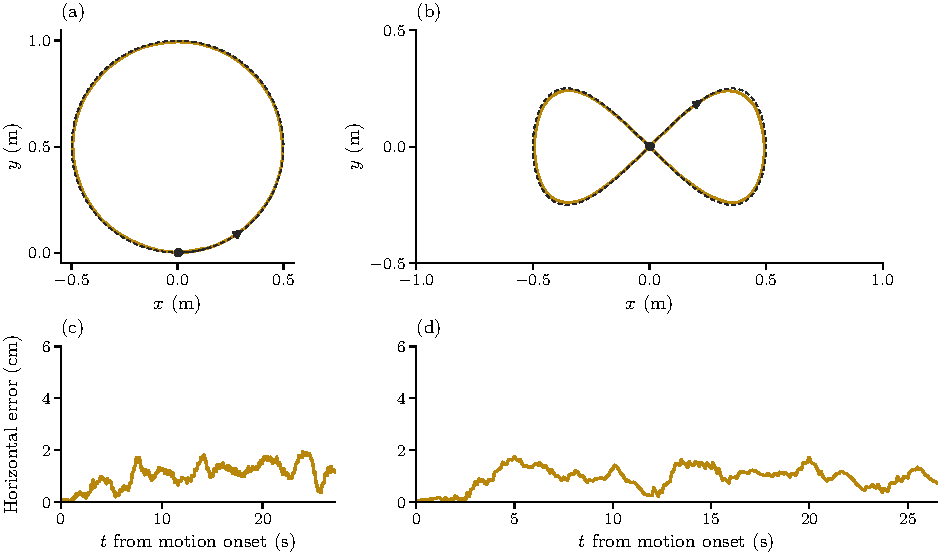
\includegraphics[width=\textwidth]{Images/trajectories.pdf}
\caption[The ring's path in the twin]{The ring's path in the rig twin at the rig's speed: three carriers, 0.125\,m/s
peak path speed, one run of each from the carry claim. (a) The orbit, one lap of radius 0.5\,m; (b) the figure-eight,
$a = 0.5$\,m. Gold: the ring's centre; dashed: the path; dot and arrow: start and direction. (c, d) The ring's
horizontal distance from the planner's reference, sampled at its 10\,Hz updates, from the onset of motion; this
time-indexed error includes the lag, which Table~\ref{tab:T7t} reports apart.}
\label{fig:traj}
\end{figure}

\begin{figure}[htbp]
\centering
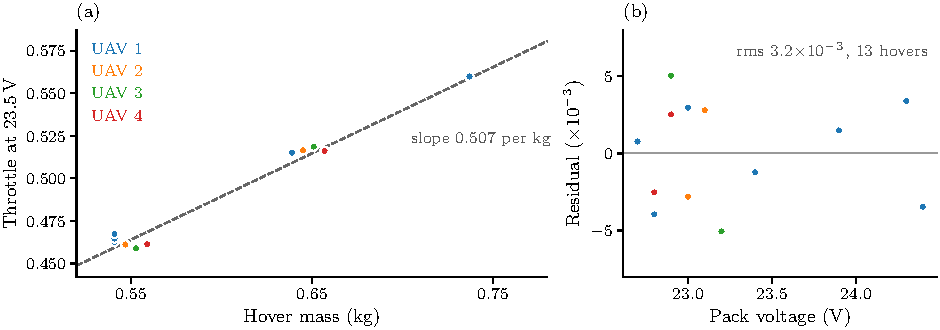
\includegraphics[width=\textwidth]{Images/thrust_map.pdf}
\caption[The rig's thrust map]{The rig's thrust map from 13 free hovers on 30 September, each UAV carrying 0, 98 or
196\,g. (a) Hover throttle corrected to 23.5\,V and to the mean offset, against the hover mass; one colour per UAV
(markers offset sideways by up to 9\,g so that hovers at the same mass can be seen); dashed: the fit
\eqref{eq:thrust_fit} with per-UAV offsets $a_i$ of 0.181--0.187. (b) The residuals of the fit against the pack
voltage: rms $3.2\times10^{-3}$, at most $5\times10^{-3}$ (about 1\,\% of hover throttle), with no trend left in
voltage.}
\label{fig:thrust_map}
\end{figure}

\begin{figure}[htbp]
\centering
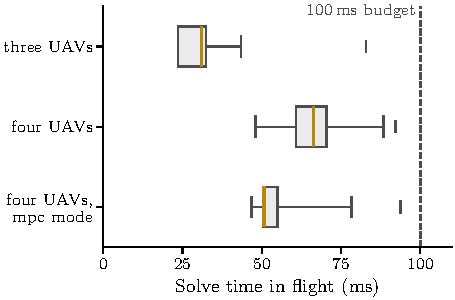
\includegraphics{Images/solve_time.pdf}
\caption[Planner solve time on the rig]{The planner's optimisation time in flight on the rig, 7--8 October:
three UAVs (after a detach, 15\,883 ticks), four UAVs (detach mode, 4\,762 ticks; carry mode, 22\,385 ticks). Box:
quartiles and median (gold); whiskers: 1st and 99th percentile; bar: the slowest tick. Medians 31, 66 and 51\,ms;
99th percentiles 44, 88 and 78\,ms; no tick reached the 100\,ms tick (dashed).}
\label{fig:solve_time}
\end{figure}

\begin{figure}[htbp]
\centering
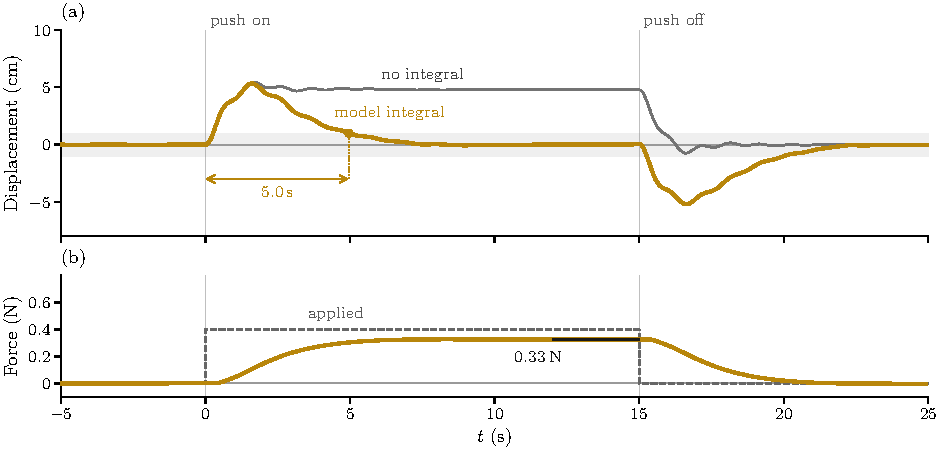
\includegraphics[width=\textwidth]{Images/disturbance.pdf}
\caption[Rejection of a horizontal force on the ring]{Rejection of a constant horizontal force on the ring in the
rig twin: three carriers, hover at 1.0\,m, the measured rod pull; a 0.4\,N push acts from 0 to 15\,s; one run of
each case (Table~\ref{tab:disturbance} gives both runs and the vertical push). (a) Ring displacement along the push,
relative to its mean over the 5\,s before: no integral (grey) and the integral in the planner's model (gold). Band:
$\pm 1$\,cm. Arrow: the time for the model integral to bring the ring back within 1\,cm for good. (b) Change of the
model integral's force $\mathbf{d}$ along the push from its value before the push (gold), against the applied force
(dashed). Black bar: its mean over the last 3\,s of the push.}
\label{fig:disturbance}
\end{figure}

\subsection{Releases on the rig}

\begin{table}[htbp]
  \centering
  \footnotesize
  \caption[The rig release record: conditions]{The hardware release record, conditions (T8a): one row per release
  event, the uncommanded ones included. Layout: the survivors' plates, then the leaver's, and the largest gap left.
  L10 and L11 are the uncommanded releases of the attach flights of 14 and 15 October, with three carriers and the
  fourth UAV not yet attached; they are not yet scored on the frozen metric. [L8 and L9: the next rig day.]}
  \label{tab:T8a}
  \begin{tabularx}{\textwidth}{lYccYYY}
    \toprule
    Event & Release & Pull source & Rod plan & Integral & Layout, largest gap & Freed-UAV policy \\
    \midrule
    L1 & announced & planned & 45$^\circ$ & reference & 3/7/11 + 9, 120$^\circ$ & hovers in place; lands with the fleet \\ % r0012 (7 Oct): no step-out
    L2 & announced, then two uncommanded & planned & 45$^\circ$ & reference & 3/6/11 + 9, 150$^\circ$ & steps out 0.5\,m \\ % r0013 (7 Oct): the rods at 11 and 6 let go 0.17 and 0.39 s after the release; capsize
    L3a & uncommanded, circle & measured & 45$^\circ$ & model & 0/6/9 + 3, 180$^\circ$ & none (carry planner); operator LAND \\ % r200006 slip 1 (7 Oct), four UAVs on the even ring, the rod at plate 3 let go 3.9 s into the orbit
    L3b & uncommanded, in the landing & measured & 45$^\circ$ & model & 0/9 + 6, 270$^\circ$ & none \\ % r200006 slip 2, 2.8 s after slip 1; capsize
    L4 & announced & measured & 60$^\circ$ & reference & 3/7/11 + 9, 120$^\circ$ & steps out 0.5\,m; lands with the fleet \\ % r302_3 (8 Oct), detach_drop.yaml, drop_on_loss armed
    L5 & unannounced & measured & 60$^\circ$ & reference & 3/7/11 + 9, 120$^\circ$ & steps out 0.5\,m; lands with the fleet \\ % r303_4 (8 Oct), drop_and_land.yaml, detect 0.06 m
    L6 & unannounced & measured & 60$^\circ$ & reference & 3/6/11 + 9, 150$^\circ$ & steps out 0.5\,m; lands with the fleet \\ % r304_3 (8 Oct)
    L7 & unannounced, circle & measured & 60$^\circ$ & reference & 3/7/11 + 9, 120$^\circ$ & clears the orbit, lands alone \\ % r305 (8 Oct), departed_land
    L8 & unannounced & measured & 60$^\circ$ & model & 3/7/11 + 9, 120$^\circ$ & lands, disarmed alone \\
    L9 & unannounced, circle & measured & 60$^\circ$ & model & 3/7/11 + 9, 120$^\circ$ & lands, disarmed alone \\
    L10 & uncommanded, in the lift & measured & 60$^\circ$ & model & three carriers, one lost & none: the drop rule was then off in this mode \\ % RIG-1014-t5_2
    L11 & uncommanded, in hover & measured & 60$^\circ$ & model & 3/11 + 7, two left & the drop rule: every carrier lands \\ % RIG-1015-a2_2: QUAD2 let go of plate 7
    \bottomrule
  \end{tabularx}
\end{table}

\begin{figure}[htbp]
\centering
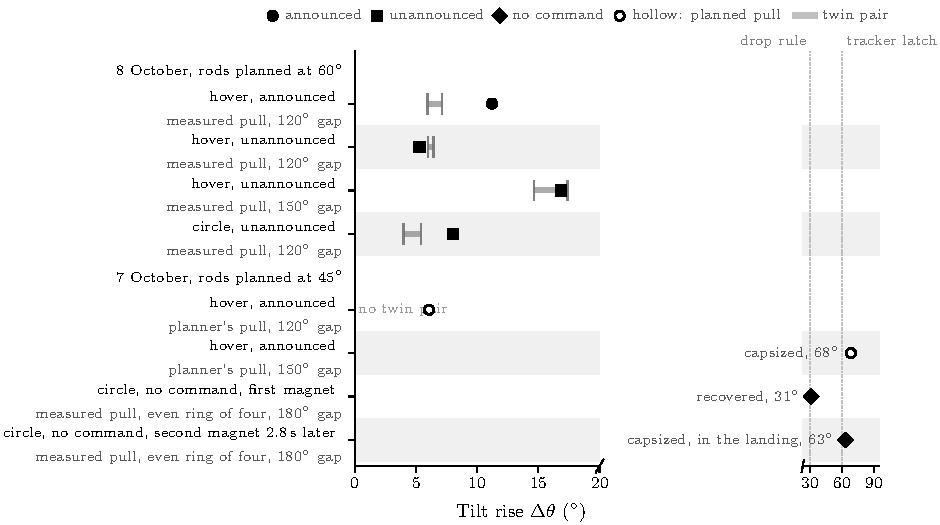
\includegraphics[width=\textwidth]{Images/releases.pdf}
\caption[Every release on the rig]{Every release on the rig to 8 October, one row per event, grouped by the day and
the rod plan: the ring's tilt rise $\Delta\theta$ (the departure of its tilt vector from its mean over the 5\,s
before the event, over the event to LAND or to the fleet's latch) as a marker, filled for the measured rod pull and
hollow for the planner's pull, shaped by how the release came (announced, unannounced, or a magnet letting go with no
command); the grey bar with end ticks is the range of the twin pair flown on the same configuration, cut at the rig
flight's hold, and rows without one say so. The two capsizes and the one recovery sit on the broken axis against the
30$^\circ$ drop rule, which these flights predate, and the trackers' 60$^\circ$ latch. The 7 October circle flew the
even ring of four, whose three survivors leave a 180$^\circ$ gap; it lost two magnets 2.8\,s apart, recovered from the
first, and capsized on the second during the landing, so that row's pre-window holds the first recovery.}
\label{fig:F10}
\end{figure}

\begin{figure}[htbp]
\centering
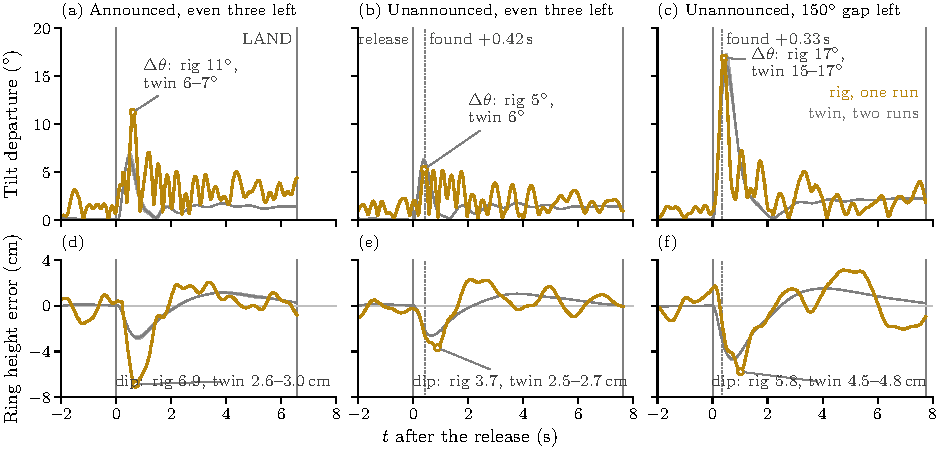
\includegraphics[width=\textwidth]{Images/rig_detach.pdf}
\caption[Releases on the rig against the twin]{Releasing one UAV of four on the rig, 8 October (gold, one run each)
against the rig twin (grey band and line: two runs, nearly identical), aligned on the release (dotted). Announced: the
planner releases the magnet and drops the UAV from its optimisation at once. Unannounced: the magnet is switched off
without telling the planner, which finds the release from the stretched rod (second dotted line, 0.33--0.42\,s after
the release on the rig). (a--c) The ring's tilt departure: the length of its tilt vector's difference from that
vector's mean over the 5\,s before the release, so that the rig ring's own rocking in hover (1--1.4$^\circ$ about its
mean) is measured about the mean rather than added to the rise; the marker and label give the tilt rise
$\Delta\theta$, the departure's peak from the release to LAND, with the twin cut at the rig flight's hold. (d--f) Ring
height error, measured minus planned (negative: below). Announced: the rig rose 11$^\circ$ against the
twin's 6--7$^\circ$, and its lowest height error was 6.9\,cm against 2.6--3.0\,cm. Unannounced: the rig rose
5$^\circ$ against 6$^\circ$ and 17$^\circ$ against 15--17$^\circ$, and its lowest height error was about 1\,cm
lower than the twin's (3.7 against 2.5--2.7\,cm; 5.8 against 4.5--4.8\,cm). (Table~\ref{tab:T8b} measures the dip
against the pre-event mean instead.) Rig traces end at the fleet's LAND.}
\label{fig:rig_detach}
\end{figure}

\paragraph{Against the rig's no-event floor.} With nothing happening, the same statistic over a 7\,s hover window
reads 4.8$^\circ$ on average across 23 such windows (95th percentile 6.0$^\circ$) and 6.3$^\circ$ over a 15\,s path
window (43 windows, 8.3$^\circ$), because it takes the largest excursion of a two-dimensional vector over the window.
L4 and L6 lie above every no-event window. On raw $\Delta\theta$, L5 lies inside the hover null and L7 inside the
path null. Scaled by each window's own pre-event rocking, L1 and L7 do not separate from it, L5 does
(4.5\,$\sigma_\mathrm{pre}$ against a null median of 3.3). [The hover null rests on two 7 October carry flights; the
path null mixes the planned and the measured pull.] L1's absolute peak came 0.1\,s before LAND; its first second
peaked at 4.6$^\circ$, and its $\Delta\theta$ exceeds its peak because the tilt swung to the far side of a
1.5$^\circ$ pre-event lean.


\subsection{One release in the twin}
\label{sec:res_twin_release}

Figure~\ref{fig:detach} shows one unannounced hover release in the twin on the freeze code tree, the cell the rig's
next hover release flies: four UAVs on plates 3, 7, 9 and 11, the magnet on plate 9 switched off without telling the
planner, the measured pull and the model integral. The planner finds the loss from the stretched rod and, re-solved
for the three survivors on their actual plates, hands the released UAV's share to them in one tick: the three end
equal, as the statics of the even triangle say (Section~\ref{sec:reconfig}). Over the three runs of this arm (the
release moved by 0.5\,s between them, so only the first is exactly the rig cell's configuration) the tilt rise was
5.5--7.7$^\circ$, the ring dipped 2.7--3.8\,cm, it was back in its band (Section~\ref{sec:metrics}) 3.9--4.2\,s after
the release, and every run landed with the freed UAV disarmed alone.

\begin{figure}[htbp]
\centering
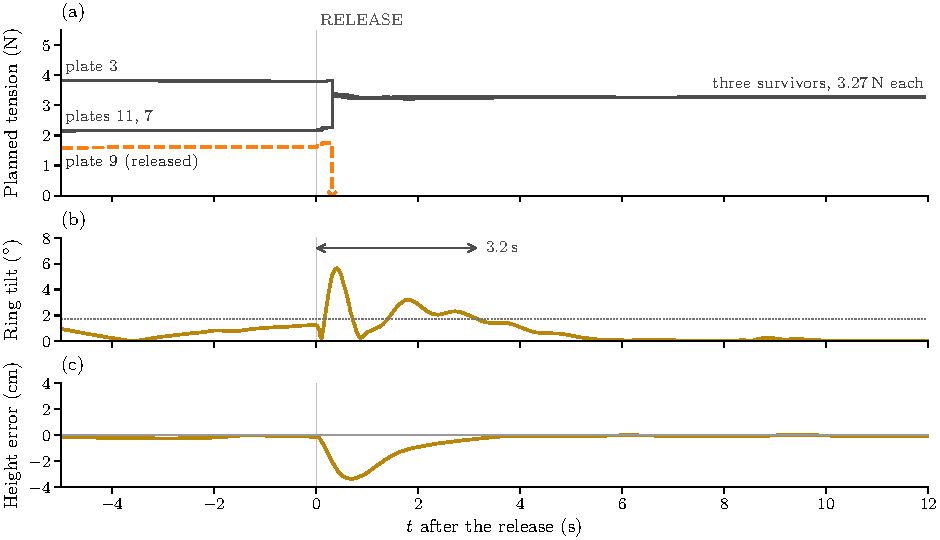
\includegraphics[width=\textwidth]{Images/detach.pdf}
\caption[One release in the twin]{An unannounced release of one UAV of four in the rig twin, hover at 1.0\,m, UAVs on
plates 3, 7, 9 and 11 (Figure~\ref{fig:geometry}), the measured rod pull and the model integral; one run. (a) The
rod tension planned for each UAV; the UAV on plate 9 (dashed) is released at RELEASE and dropped from the plan when the
planner finds the loss, and the three survivors, now an even triangle, share the load equally. (b) Ring tilt; dotted:
the hover's own maximum plus 0.5$^\circ$; arrow: the time until the tilt stays below it. (c) Ring height error
against the 1.0\,m target. The tensions are planned, since the twin does not measure them.}
\label{fig:detach}
\end{figure}


\subsection{The freed UAV's landing}

The freed UAV's own landing, on the rig on 8 October under the old rule and in the twin under the old and the new rule
(Figure~\ref{fig:departed_landing}); the rig's own pair with the new rule waits for the next rig day
(Figure~\ref{fig:rig_departed}).

\begin{figure}[htbp]
\centering
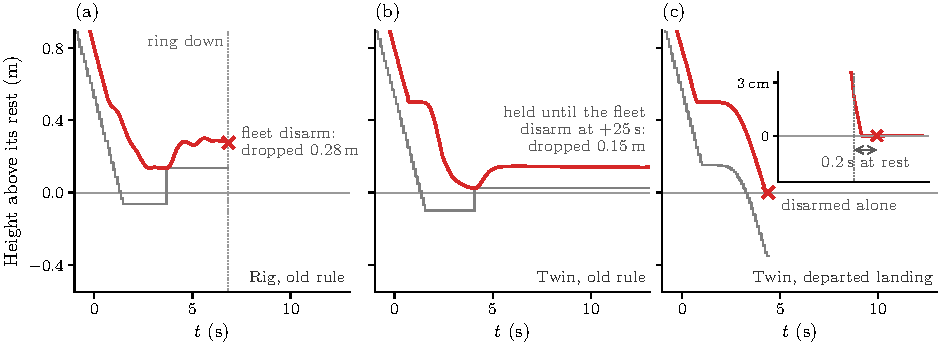
\includegraphics[width=\textwidth]{Images/departed_landing.pdf}
\caption[A freed UAV's own landing, old rule and departed landing]{A UAV landing by itself off the ring, the same UAV
(the fourth) in three cases, aligned where it passes 0.8\,m on the way down; solid: its height above its own resting
height, grey: its height reference until it is disarmed, cross: its disarm, dotted: the ring reaching the floor. (a)
Rig, old rule: its touchdown test fired 0.14\,m above its rest, the reference froze there, the UAV rose to 0.28\,m and
hovered until the fleet's disarm at the end of the landing dropped it 0.28\,m. (b) Twin, old rule: the same stall, held
0.15\,m up for 25\,s until the fleet's disarm dropped it. (c) Twin, departed landing: the reference is pressed below the
resting height until the UAV is there, and it is disarmed alone 0.2\,s after reaching it (inset). The plateau at 0.5\,m
in (b) and (c) is the UAV standing on the tip of its rod before the rod tips over.}
\label{fig:departed_landing}
\end{figure}

\pendingfig{fig:rig_departed}{The freed UAV's own landing on the rig with the departed landing: pushed to its resting
height and disarmed alone.}{the rig's hover and circle releases (L8, L9), the next rig day}

\subsection{The twin against the rig, 8 October}

\begin{figure}[htbp]
\centering
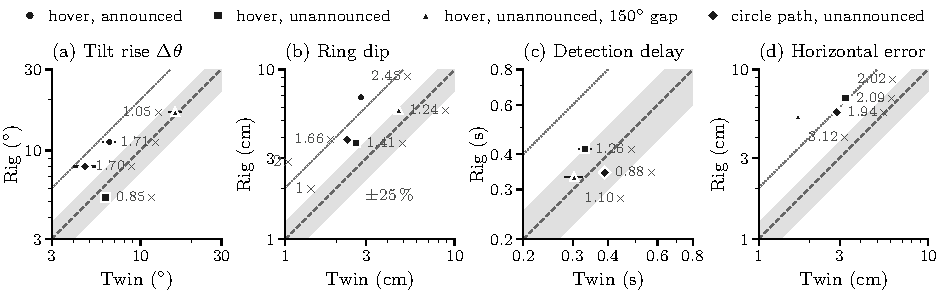
\includegraphics[width=\textwidth]{Images/twin_rig_parity.pdf}
\caption[The twin against the rig]{The rig against its twin for the four releases of 8 October (four UAVs,
0.86\,kg ring at 1.0\,m; one marker per flight; 150$^\circ$ gap: the three left on the ring leave a 150$^\circ$ gap
between two of them), each metric computed the same way from both, on logarithmic axes: $x$, the twin flying the same
configuration (mean of two runs; bar: their range, hidden where it is shorter than the marker); $y$, the rig (one run).
Dashed: $y = x$; grey band: within 25\,\% of the twin; dotted: the rig twice the twin. (a) Tilt rise $\Delta\theta$:
the peak of the ring's tilt-vector departure from its mean over the 5\,s before the release, from the release to the
rig flight's LAND, the twin cut at the same hold. (b) Ring dip: its lowest height error in the 3\,s after the release.
(c) Detection delay: from the release to the planner finding an unannounced release (an announced release needs
none). (d) Horizontal error: the ring's mean distance from its reference over the 10\,s before the release. Within
25\,\% of the twin: the tilt rise of the unannounced hover and 150$^\circ$-gap releases (0.85 and 1.05 times the twin),
the dip of the 150$^\circ$-gap release, and two of the three detection delays (the third is 1.26 times the twin; all
three within 0.1\,s). The announced hover release and the circle release rose 1.7 times the twin; the other three dips
were 1.4--2.5 times the twin's, and the horizontal error was 1.9--3.1 times (5.3--6.8\,cm against 1.7--3.3\,cm).}
\label{fig:twin_rig_parity}
\end{figure}


\section{Secondary results, negative results and history}
\label{sec:app_negatives}

\subsection{Approaches to model error on the earlier stack}
\label{sec:app_methods}

Before the tracker's initial-condition fix and the measured rod pull, five approaches to model error were flown in
the three-UAV twin against the hover, one UAV's thrust map wrong in either direction, a 1\,N push and a 0.4\,m/s wind
(Table~\ref{tab:methods}). Three cases represent the internal errors: the hover itself, and one UAV whose thrust map
is wrong in each direction (its real offset 0.03 above or below the 0.185 its tracker assumes). Two represent external
forces: a 1\,N horizontal push on the ring, and a 0.4\,m/s wind during the orbit. All of them were flown with the
tracker's relaxed initial condition, so the hover without any correction sits 4.8\,cm high; the comparisons between
rows still hold, and the measured cable force of this table is the one that became the trackers' measured pull.

\begin{table}[h]
\centering
\footnotesize
\setlength{\tabcolsep}{4pt}
\caption{Approaches to model error in the Gazebo rig twin (three UAVs, 1.0\,m, floor start; flown
with $\epsilon = 0.025$). Height and horizontal errors in cm, tilt in degrees; one run per cell
unless noted; a dash: not flown. $^{a}$ A UAV tipped during the landing, after the hover, and the fleet
disarmed. $^{b}$ Two runs, agreeing within 0.1.}
\label{tab:methods}
\begin{tabular}{lccccc}
\toprule
 & Hover & One UAV weaker & One UAV stronger & 1\,N push & Wind \\
 & $e_z$ & $e_z$ / $e_{xy}$ / tilt & $e_z$ / $e_{xy}$ / tilt & $e_{xy}$ & $e_{xy}$ \\
\midrule
None & +4.8 & $-$3.0 / 3.8 / 6.7 & +12.8 / 3.5 / 6.0 & 18.0 & 17.9 \\
Height integral (target) & +0.1 & 0.0 / 3.8 / 6.7 & 0.0 / 3.5 / 6.0 & 17.9 & 18.0 \\
Force balance & +3.8 & +3.9 / 1.3 / 9.0 & -- & 0.3 & 3.9 \\
Force balance + height int. & +0.1$^{b}$ & 0.0 / 1.3 / 9.0$^{b}$ & -- & 0.4$^{b}$ & 3.9$^{b}$ \\
Offset-free observer & +1.6 & +1.0 / 0.2 / 8.0 & +2.4 / 0.1 / 7.5 & 2.6$^{b}$ & 7.8$^{b}$ \\
Measured cable force & +4.2$^{a}$ & +3.8 / 3.1 / 0.8$^{a}$ & +4.5 / 0.6 / 0.3 & -- & -- \\
Measured force + height int. & 0.0$^{a}$ & 0.0 / 3.1 / 0.8 & 0.0 / 0.6 / 0.3$^{a}$ & -- & -- \\
Thrust-gain trim & +3.7 & +4.1 / 1.3 / 2.3 & -- & -- & -- \\
Rod mass in the planner & +5.0 & -- & -- & -- & -- \\
\bottomrule
\end{tabular}
\end{table}

\begin{description}
    \item[Height integral on the target.] Zeroes the height in every case and does nothing
    horizontally: the push and the wind still move the ring 18\,cm.
    \item[Force balance.] Estimates a constant force on the ring and one shared by the UAVs from
    the measured motion and the delivered thrust, and gives them to the planner's model
    \cite{muske2002disturbance}. It removes the push and most of the wind. It cannot see the internal
    height offset: by Newton's law, a force that the system exerts on itself does not appear in its
    total. It books a UAV's thrust-map error as a force on the ring, and leans the formation into
    it, which tilts the ring further. Combined with the height integral it was the best on height and
    external forces. Its transients were not small: on the push it peaked at 14.5\,cm, and on release
    it overshot by 14.8\,cm and tilted the ring 7.1$^\circ$.
    \item[Offset-free observer.] Estimates the force from the planner's own prediction error, as in
    offset-free MPC \cite{pannocchia2003disturbance}. It helped everywhere but converged slowly and left
    residuals, because a small offset shows up in the plan's rod states rather than in the payload's
    predicted motion.
    \item[Measured cable force.] Each tracker takes its rod's force from its measured acceleration
    and delivered thrust, the ground-side counterpart of the compensation from inertial measurements of
    \cite{tudelft}. It was the only approach that levelled the ring against one UAV's wrong thrust
    map (0.3--0.8$^\circ$ against 6--7$^\circ$), because it corrects each UAV's own force. In four of
    six runs, however, a UAV tipped during the landing.
    \item[Thrust-gain trim.] A per-UAV estimate of the throttle-to-acceleration gain, from the UAV's
    own measured acceleration and its static share of the rod force. It partly corrects a wrong map.
    \item[Rod mass in the planner.] Corrected the rods' elevation (49.7 to 42.8$^\circ$ against a planned
    45$^\circ$) but not the height.
\end{description}
Further candidates were rejected before flying, because tests on logged flights showed they would
not work. These were pinning the rod rates at node~0, a thrust reference weight in the
tracker, and an $\mathcal{L}_1$ adaptive force estimate \cite{hovakimyan2010l1} at the planner's
10\,Hz rate. Raising the planner's weight on the ring's horizontal position by three and by ten times
cut the push displacement only by 23 and 38\,\% (18.5 to 14.3 and 11.4\,cm), and the higher weight
rocked the ring by 6$^\circ$. Aiming the rods at the hand-over angle instead of 45$^\circ$ made it
worse (20.7\,cm). Both were removed.

\subsection{Further tests in the rig twin}
\label{sec:app_tests}

\paragraph{Trajectories at the rig's speed.} Table~\ref{tab:traj} gives the three-carrier hover and the five load
paths at 0.125\,m/s from the carry claim on the planner's own 10\,Hz reference, with the height error and, for the
spin, the yaw.
\begin{table}[htbp]
\centering
\caption[Trajectories at the rig's speed]{Trajectories in the rig twin at 0.125\,m/s peak path speed: three
carriers, ring at 1.0\,m, floor start, the default controller, two runs each from the carry claim (the hover from the
model-error study's baseline). Horizontal error per sample against the planner's reference at its 10\,Hz updates, over
the motion (the orbit's first lap) or the 15\,s before LAND (hover); height error and tilt: means over the same window.
The circle starts from the lift point; the orbit is flown continuously.}
\label{tab:traj}
% generated by tools/thesis_sim_tables.py on the freeze tree (17 Oct; appendix re-fly)
\begin{tabularx}{\textwidth}{>{\raggedright\arraybackslash}Xccccccc}
\toprule
 & & Speed & \multicolumn{2}{c}{Horizontal error (cm)} & Height & Tilt & \\
\cmidrule(lr){4-5}
Reference & UAVs & (m/s) & mean & max & error (cm) & (\si{\degree}) & Runs \\
\midrule
Hover & 3 & -- & 0.0 & 0.1 & $-$0.1 & 0.1 & 2 \\
Circle, one lap, $r = 0.5$\,m & 3 & 0.125 & 0.5 & 1.4 & $-$0.1 & 0.3 & 2 \\
Orbit, first lap, $r = 0.5$\,m & 3 & 0.125 & 0.9 & 1.7 & $-$0.1 & 0.6 & 2 \\
Figure-8, $r = 0.5$\,m & 3 & 0.125 & 0.7 & 1.4 & $-$0.1 & 0.6 & 2 \\
Line, 1\,m & 3 & 0.125 & 0.5 & 1.6 & $-$0.1 & 0.3 & 2 \\
Spin, circle with one turn of yaw$^a$ & 3 & 0.125 & 0.6 & 1.7 & $-$0.1 & 0.4 & 2 \\
\bottomrule
\multicolumn{8}{l}{\footnotesize $^a$ Yaw error 1.8\,\si{\degree} mean, 3.9\,\si{\degree} max over the turn.}
\end{tabularx}

\end{table}

\paragraph{The tracker's initial condition.} Table~\ref{tab:x0} gives the means behind Section~\ref{sec:res_ic}.
\begin{table}[h]
\centering
\caption{Ring error with the relaxed and the pinned initial condition, no integral action, on the freeze code tree
(two runs each).}
\label{tab:x0}
% generated by tools/thesis_sim_tables.py on the freeze tree (17 Oct; appendix re-fly)
\begin{tabular}{llcc}
\toprule
Case & Metric & $\epsilon = 0.025$ & $\epsilon = 0$ \\
\midrule
Twin, hover at 1.0\,m & height error (cm) & +13.1 (2) & $-$0.1 (2) \\
Twin, orbit & horizontal error, mean (cm) & 3.9 (2) & 0.7 (2) \\
 & height error (cm) & +13.0 (2) & $-$0.1 (2) \\
\bottomrule
\end{tabular}

\end{table}

\paragraph{Integral gain and gate.} Table~\ref{tab:gain} gives the gain and the gate on the 0.6\,N vertical push. On
the measured pull the push hardly reaches the integral, and neither doubling the gain nor keeping the speed gate only
for the first 5\,s after the lift makes a difference the resolution rule resolves.
\begin{table}[h]
\centering
\caption{Integral gain and gate on the 0.6\,N vertical push, model integral, the measured pull. Peak: largest
displacement during the push; overshoot and settling (to within 1\,cm): after it ends. Brackets: number of runs.}
\label{tab:gain}
% generated by tools/thesis_sim_tables.py on the freeze tree (17 Oct; appendix re-fly)
\begin{tabularx}{\textwidth}{Xccc}
\toprule
Model integral & Peak (cm) & Overshoot (cm) & Settling (s) \\
\midrule
$k_i = 0.4$ & 1.3 (2) & 1.4 (2) & 1.2 (2) \\
$k_i = 0.8$ & 1.3 (2) & 1.3 (2) & 1.1 (2) \\
$k_i = 0.4$, speed gate only in the first 5\,s after the lift & 1.3 (2) & 1.3 (2) & 1.1 (2) \\
\bottomrule
\end{tabularx}

\end{table}

\paragraph{Landings.} Table~\ref{tab:land} gives every landing of the freeze code tree in the rig twin
(Section~\ref{sec:sim_landing}). The re-armed touchdown test was flown afterwards on its own card: on the rig's
landing path with correct thrust maps the false touchdown came in 2 of 4 runs without it and 0 of 5 with it; with one
UAV's throttle offset 0.03 below its map's (about 1\,m/s$^2$ of surplus thrust) it removed the 0.4--0.5\,m case but left that UAV 15.7--15.8\,cm above its rest at the
disarm, leaning 24--30$^\circ$ on its rod afterwards (eight runs).
\begin{table}[h]
\centering
\caption{Every landing of the freeze code tree in the rig twin, from load-down until the fleet is declared landed and
after it.}
\label{tab:land}
% generated by tools/thesis_sim_tables.py on the freeze tree (17 Oct), then edited by hand per the reviewer of the
% appendix re-fly: the generator stopped at LANDED and missed the false touchdowns (R2032, R2044, R2045 at 0.46-0.53 m;
% R2033 one UAV at 0.26 m), so the "disarmed in the air" column is added; the straight-descent row is the freeze
% tree's L-S pair (R2049, R2064). "+" = outside the reference.
\begin{tabularx}{\textwidth}{>{\raggedright\arraybackslash}Xcccc}
\toprule
Landing & Runs & Disarmed in the air$^a$ & Pushed outward (cm) & Tilt after 1.2\,s (\si{\degree}) \\
\midrule
straight descent & 2 & 0 & 23.5--23.6 & 6.8--12.4 \\
unwind, feedforward ramp, ground idle & 82 & 4$^b$ & $-$2.2--0.6 & 1.5--4.7 \\
\bottomrule
\multicolumn{5}{p{0.95\textwidth}}{\footnotesize $^a$\,The fleet declared landed and disarmed with a UAV more than
0.2\,m above its rest. $^b$\,All four with one UAV stronger than its thrust map: in three every UAV was
0.46--0.53\,m up and fell onto its side, in the fourth one UAV was 0.26\,m up. In the other 78 no UAV was disarmed
more than 0.05\,m above its rest. The pushed-outward and tilt columns end when the fleet is declared landed.}
\end{tabularx}

\end{table}

\subsection{Wrong model values}
\label{sec:app_robust}

Table~\ref{tab:robust} gives the twin's hover at 1.0\,m, three UAVs from a floor start, with one wrong value in the
controller while the simulated rig keeps the true ones, each case flown without and with the integral
(Section~\ref{sec:sim_robustness}). The rows tested on the earlier stack that this table does not have (rods typed
short, the radius typed short, and the combination with a mass error) were not re-flown.
\begin{table}[htbp]
\centering
\caption[Hover with a wrong model]{Hover at 1.0\,m with one wrong value in the controller's model, rig twin, three
UAVs, $\epsilon = 0$, the measured pull, floor start, freeze code tree. Height error: the mean of two runs over the 15\,s
before LAND. Integral force at LAND: the vertical component. Tilt: mean over the four runs. Landed: flights that
landed without a fault.}
\label{tab:robust}
% generated by tools/thesis_sim_tables.py on the freeze tree (17 Oct; appendix re-fly R2023, R2035, R2034, R2046,
% R2050-R2061, R2065-R2076), then edited by hand per the reviewer (docs/analysis/appendix_refly_2026-10-17.md): the
% "learned force" column relabelled as the integral's force at LAND with footnote c (wind-up, not learned), footnote a
% rewritten (no error left for the gate; the planned-pull pair R2085/R2087 +22.2 cm), footnote b kept (C-R2).
\begin{tabularx}{\textwidth}{>{\raggedright\arraybackslash}Xccccc}
\toprule
 & \multicolumn{2}{c}{Height error (cm)} & Integral force & & \\
\cmidrule(lr){2-3}
Error in the controller's model & no integral & integral & at LAND (N) & Tilt (\si{\degree}) & Landed \\
\midrule
none & $-$0.1 & $-$0.1 & $-$0.05 & 0.1 & 4/4 \\
payload mass typed $+10$\,\% & 0.0 & 0.0 & $-$0.03 & 0.1 & 4/4 \\
payload mass typed $+20$\,\% & 0.0$^a$ & 0.0 & 0.00 & 0.1 & 4/4 \\
payload mass typed $-20$\,\% & $-$0.1 & $-$0.1 & $-$0.10 & 0.1 & 4/4 \\
rods typed $+5$\,cm, measured at the hand-over & $-$0.1 & $-$0.1 & $-$0.05 & 0.1 & 4/4 \\
rods typed $+5$\,cm, not measured & $+$17.1 & $+$17.1$^b$ & 0.00 & 0.1 & 4/4 \\
attachment radius typed $+2$\,cm & $+$0.9 & $+$0.9 & 0.76$^c$ & 0.1 & 4/4 \\
\bottomrule
\multicolumn{6}{p{0.95\textwidth}}{\footnotesize $^a$\,On the planner's pull instead of the measured pull, the same
error left $+22.2$\,cm (exploratory pair). $^b$\,The unmeasured rods read as partly slack, so the integral's
tautness gate stays closed. $^c$\,Not a learned force: the vertical integral winds up through the hold while the
height error stays where it is without the integral.}
\end{tabularx}

\end{table}

\subsection{The levers on a release, pair by pair}
\label{sec:app_levers}

Table~\ref{tab:T9} gives every lever pair flown on the detach freeze code tree with its frozen sign, its label and its
verdict under the resolution rule of Section~\ref{sec:metrics}: the sign as frozen, the ranges apart, and the gap at
least the larger of the floor and twice the larger range.

\begin{table}[htbp]
\centering
\footnotesize
\setlength{\tabcolsep}{3pt}
\caption[The lever pairs]{The lever pairs on a release in the twin (T9): unannounced hover releases unless stated, the
model integral, every link rigid. Values: $\Delta\theta$ ($^\circ$), the arm mean and [range]; $\geq$: a lower bound cut
at the drop or the latch. Needed: max(floor, twice the larger range). Labels: R, replication; N, new prediction.
$^a$\,The tool's reading counts the freed UAV, which with detection off stays in the formation; on the three UAVs still
on the ring, 1.37 against 1.80$^\circ$, unresolved. $^b$\,Mean path error on the even ring's 60$^\circ$ circle (cm),
floor 0.3\,cm. $^c$\,The drop rule off at 180$^\circ$, declared before the runs, so the pair also differs in that setting,
and the $\geq$ values are the 60$^\circ$ latch that exists only with it off; on the default rules the gap rule dropped
the ring at detection ($\geq$24.08$^\circ$). $^d$\,Falsified as written by the planner's pull at 150$^\circ$ (both runs at the
drop line); every measured-pull peak was under 30$^\circ$ (largest 16.9$^\circ$).}
\label{tab:T9}
\begin{tabularx}{\textwidth}{>{\raggedright\arraybackslash}X>{\raggedright\arraybackslash}p{1.7cm}c>{\raggedright\arraybackslash}p{1.85cm}>{\raggedright\arraybackslash}p{1.85cm}>{\raggedright\arraybackslash}p{1.2cm}>{\raggedright\arraybackslash}p{1.7cm}}
\toprule
Pair (one variable) & Frozen sign & Label & Arm A & Arm B & Gap / needed & Verdict \\
\midrule
Pull source, 120$^\circ$ gap & measured $<$ planned & N & 6.40 [5.46, 7.68] & 16.80 [16.64, 17.08] & 10.40 / 4.44 & confirmed \\
Detection, planner's pull & on $<$ off & N & 16.80 [16.64, 17.08] & 28.18 [28.17, 28.20] & 11.38 / 1.00 & confirmed \\
Detection, measured pull & no sign & R & 6.40 [5.46, 7.68] & 5.58 [4.64, 6.66] & $-$0.82 / 4.44 & confirmed (no sign) \\
Landing lean, detection, measured pull & on $<$ off & N & 1.37 [1.2, 1.6] & 4.80 [4.7, 4.9] & 3.43 / 1.00 & not credited$^a$ \\
Landing lean, detection, planner's pull & on $<$ off & N & 1.90 [1.8, 2.0] & 4.23 [3.4, 5.4] & 2.33 / 4.00 & unresolved \\
Pull source, 60$^\circ$ circle, no event$^b$ & planned $<$ measured & R & 0.53 [0.49, 0.58] & 0.93 [0.87, 0.98] & 0.39 / 0.30 & confirmed, even ring, $n = 2$ \\
\midrule
Margin 112 to 58\,mm (gap 120 to 150$^\circ$) & smaller margin, larger & R & 6.40 [5.46, 7.68] & 16.82 [16.65, 16.99] & 10.42 / 4.44 & confirmed \\
Margin 58 to 0\,mm (150 to 180$^\circ$)$^c$ & smaller margin, larger & N & 16.82 [16.65, 16.99] & $\geq$61.22 [60.71, 61.72] & 44.40 / 2.02 & confirmed \\
Margin 112 to 86\,mm & smaller margin, larger & N & 6.40 [5.46, 7.68] & 8.44 [7.81, 9.07] & 2.04 / 4.44 & unresolved, right sign \\
Margin 86 to 58\,mm & smaller margin, larger & N & 8.44 [7.81, 9.07] & 16.82 [16.65, 16.99] & 8.38 / 2.52 & confirmed \\
Margin 58 to 29\,mm & smaller margin, larger & N & 16.82 [16.65, 16.99] & 28.02 [27.93, 28.12] & 11.20 / 1.00 & confirmed \\
Pull source, 150$^\circ$ gap & measured $<$ planned & N & 16.82 [16.65, 16.99] & $\geq$29.54 [28.46, 30.61] & 12.71 / 4.30 & confirmed \\
Every absolute peak under 30$^\circ$, gaps 120--150$^\circ$ & -- & -- & \multicolumn{3}{>{\raggedright\arraybackslash}p{5.3cm}}{the planner's pull at 150$^\circ$ reached the drop line in 2 of 2} & falsified$^d$ \\
\bottomrule
\end{tabularx}
\end{table}

\subsection{The carry bands for the next rig day}
\label{sec:app_bands}

Table~\ref{tab:bands1m} gives the bands frozen on 17 October for the carry cells on 1\,m cables, under the rule of
Section~\ref{sec:ledger}: three twin runs per cell, $2\sigma_{\mathrm{rig}}$ of 20.6\,mm and 3.0$^\circ$, no class
factor, both metrics from the path's start to LAND.

\begin{table}[htbp]
\centering
\footnotesize
\caption[The frozen carry bands, 1\,m cables]{The frozen carry bands for the next rig day: three carriers on 1\,m
cables, the 0.86\,kg ring at 1.0\,m, three twin runs per cell. Path RMSE: the ring's distance from its published
reference; tilt: the peak ring tilt. A rig flight is scored only against a band frozen before it.}
\label{tab:bands1m}
\begin{tabular}{llcccc}
\toprule
 & Speed & \multicolumn{2}{c}{Path RMSE (mm)} & \multicolumn{2}{c}{Peak tilt ($^\circ$)} \\
\cmidrule(lr){3-4}\cmidrule(lr){5-6}
Path & (m/s) & twin runs & band & twin runs & band \\
\midrule
Circle & 0.125 & 8.3, 9.3, 8.3 & 0.0--29.9 & 1.77, 1.49, 1.67 & 0.00--4.76 \\
 & 0.2 & 11.7, 11.5, 11.0 & 0.0--32.3 & 1.72, 1.57, 1.57 & 0.00--4.72 \\
 & 0.3 & 13.4, 15.9, 19.4 & 0.0--40.0 & 1.94, 2.88, 3.94 & 0.00--6.94 \\
Figure-eight & 0.125 & 10.1, 15.0, 13.6 & 0.0--35.6 & 1.14, 1.72, 1.44 & 0.00--4.72 \\
 & 0.2 & 14.4, 16.4, 17.0 & 0.0--37.6 & 2.34, 1.66, 1.56 & 0.00--5.34 \\
 & 0.3 & 16.4, 20.9, 21.4 & 0.0--42.0 & 3.02, 3.31, 2.97 & 0.00--6.31 \\
Line & 0.125 & 5.0, 6.5, 9.1 & 0.0--29.7 & 0.97, 1.22, 1.60 & 0.00--4.59 \\
 & 0.2 & 11.2, 9.6, 9.7 & 0.0--31.8 & 3.01, 1.65, 1.64 & 0.00--6.00 \\
 & 0.3 & 13.8, 14.8, 18.7 & 0.0--39.3 & 2.18, 2.81, 3.81 & 0.00--6.81 \\
Orbit & 0.125 & 7.0, 9.8, 9.5 & 0.0--30.4 & 1.13, 1.46, 1.78 & 0.00--4.78 \\
 & 0.2 & 11.5, 12.6, 14.3 & 0.0--34.9 & 1.77, 1.76, 1.54 & 0.00--4.77 \\
 & 0.3 & 23.0, 21.5, 24.3 & 0.9--44.9 & 2.81, 3.30, 4.39 & 0.00--7.39 \\
Spin & 0.125 & 9.2, 13.5, 12.5 & 0.0--34.1 & 1.60, 3.30, 2.73 & 0.00--6.30 \\
 & 0.2 & 11.6, 16.5, 20.6 & 0.0--41.2 & 2.18, 3.35, 5.25 & 0.00--8.25 \\
 & 0.3 & 17.8, 18.3, 25.4 & 0.0--46.0 & 4.95, 4.14, 6.16 & 1.14--9.15 \\
\bottomrule
\end{tabular}
\end{table}
% docs/experiments/2026-10-16_bands_1m.md, frozen 17 Oct ~19:54 (tools/n2_bands.py; results/analysis/n2_bands_2026-10-17.json).

\subsection{Corner cutting and the timing fix}
\label{sec:app_corner}

The ring's cut at speed (Section~\ref{sec:res_envelope}) was studied on the 0.3\,m/s cells, exploratory throughout.
Raising the planner's weight on the ring's position, loosening its pull towards the flatness rod directions, or
freeing the rods' angular rate did not remove the cut in the one or two runs each arm had. What removes it is timing: shifting the trackers' references by the age of the plan they fly, with two SQP
iterations per tick and the planner's clock lead reduced by 0.075\,s (to 0.025\,s), took the figure-eight's cut at its tight bends
from 20--33\,mm to between $-$9 and +16\,mm, scattering across sessions, and centred the circle and the orbit on their
schedule. The same lead did
not hold on the spin: the lag there ran ahead in 2 of 3 pairs. A test of whether the needed shift is the loop's delay failed (0.035\,s more delay moved
it by about 0.003\,s), so the cut's source is open; a lead chosen per shape would be a band-aid, so the defaults stay
and the lag is reported. The frozen path RMSE does not see any of this, because it scores against the held
10\,Hz reference (Section~\ref{sec:metrics}).
% Sources: docs/experiments/2026-10-16_corner_cutting.md (closed 17 Oct, Wesley ~19:45: defaults stay, lag reported);
% 2026-10-17_lead075_default.md (N5 fails on spin in 2 of 3 pairs; exploratory).

\subsection{Fault coverage}
\label{sec:app_faults}

Table~\ref{tab:faults} gives, for each fault and phase, the exit that covers it and where that exit has flown.
Figure~\ref{fig:land_phases} presses LAND in every phase in the twin, and Figure~\ref{fig:disarm_lanes} shows who is
disarmed when.

\begin{table}[htbp]
\centering
\footnotesize
\caption[Fault coverage]{Fault coverage: each fault and phase, the exit that covers it, and where it has flown. Twin
evidence on the code tree named; rig evidence as flown.}
\label{tab:faults}
\begin{tabularx}{\textwidth}{>{\raggedright\arraybackslash}p{3.2cm}>{\raggedright\arraybackslash}p{2.6cm}>{\raggedright\arraybackslash}X>{\raggedright\arraybackslash}X}
\toprule
Fault, phase & Exit & Twin & Rig \\
\midrule
One carrier lost, unannounced & detect, resize; the freed UAV lands and is disarmed alone & freeze tree: carried in every run; freed UAV disarmed alone 0.27--0.43\,s after reaching its rest (5 runs) & 8 October: three carried through (the freed UAV's landing then stalled, old rule) \\
A loss leaving fewer than three, or a gap of 180$^\circ$ or more & drop the ring, land every UAV & freeze tree: dropped 0.22--0.23\,s after the loss, all down in 8.5--8.9\,s (4 runs) & 15 October: the loss left two carriers, but the tilt rule fired first (next row) \\
Ring tilt over 30$^\circ$ & drop the ring, land every UAV & freeze tree: the planner's pull at a 150$^\circ$ gap, dropped in 2 of 2, all landed & 15 October: fired at 36.8$^\circ$ after an uncommanded release; every carrier landed and was disarmed alone \\
Carrier loss with the drop rule off & fleet disarm in the air & freeze tree, 180$^\circ$ gap: latched at 60$^\circ$, disarm 1.45--1.62\,m up (2 runs) & 14 October: fleet disarmed about 1\,m up; the drop rule on in every mode since \\
Newcomer fault in transit & newcomer disarmed alone, carriers land & 9 October tree: 2 of 2 (Figure~\ref{fig:disarm_lanes}a) & not flown \\
Newcomer tilting while free & tilt cut & current tree: 4 of 4 (exploratory) & off \\
Nothing confirmed, or the collaborator gives up & take-back & the contact-and-lift tree (12 October); [the join code tree] & 15 October: a LAND in the match phase ended in a take-back, all landed \\
Ring dropped while the collaborator flies the newcomer & take-back on the drop tick & 16 October: taken back on the drop tick and down at its rest 14--17\,s later with no fault; one run failed a bar that did not fit a drop at the plate, and two pass only on a revised bar (reviewed, twin only) & on through a parameters file; not yet exercised \\
LAND in any phase & every UAV lands & 9 October tree: 33 of 34 (Figure~\ref{fig:land_phases}) & flown in carry, release and attach flights \\
Touchdown read too early & re-armed touchdown test & 0 of 5 false touchdowns with it, 2 of 4 without (rig landing path) & after review \\
\bottomrule
\end{tabularx}
\end{table}

\begin{figure}[htbp]
\centering
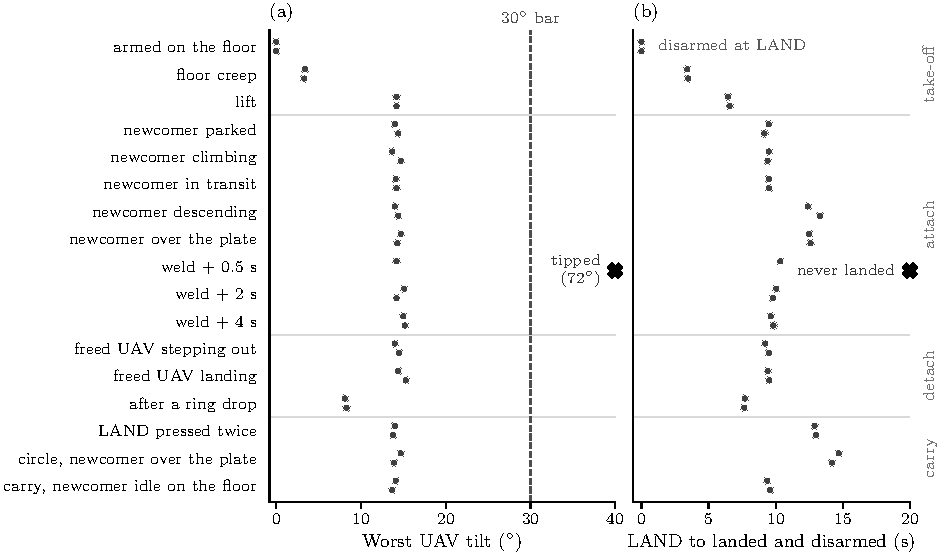
\includegraphics[width=\textwidth]{Images/land_phases.pdf}
\caption[LAND in every phase of a flight]{LAND pressed in each phase of a flight in the rig twin, two runs per
phase on the code tree of 9 October, before the collaborator's controller flew the attach and before the co-motion
confirmation (the attach phases, ``weld'' included, are of that earlier sequence). (a) The largest tilt of any UAV
between LAND and its disarm, against the 30$^\circ$ bar. (b) The time from LAND until the fleet is landed and disarmed.
Every UAV landed and was disarmed in 33 of 34 runs, within 15\,s and with no UAV past 16$^\circ$. In the other run
(LAND 0.5\,s after the newcomer's weld) the newcomer, on the twin's rigid rod, tipped while the carriers unwound after
the ring was down, and the fleet stopped; its tilt is drawn at the edge of the axis with its value. Armed on the floor,
LAND disarms the fleet at once.}
\label{fig:land_phases}
\end{figure}

\begin{figure}[htbp]
\centering
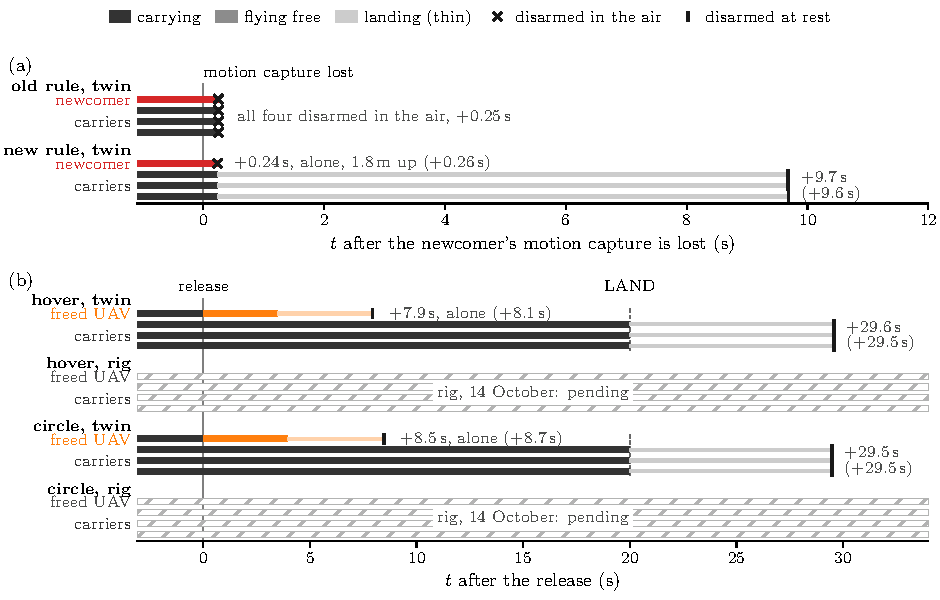
\includegraphics[width=\textwidth]{Images/disarm_lanes.pdf}
\caption[Who is disarmed when]{Which UAV is disarmed when, one lane per UAV: dark, carrying the ring; mid (or the
UAV's own colour), flying off it; light and thin, landing; cross, disarmed in the air; bar, disarmed at rest. The UAV
off the ring is drawn in its own colour once it is off, the carriers in grey; times in brackets are the repeat run's.
(a) The newcomer loses its motion capture 2\,s into its transit to the ring, in the twin. Old rule (one run): its pose
timeout disarms it and the fleet-wide stop disarms all four in the air, 0.25\,s after the loss. New rule (a fault on
the newcomer lands the fleet; two runs): it alone is disarmed, 0.24\,s after the loss and 1.8\,m above its rest, and
the carriers land the ring at once and are disarmed at rest 9.7\,s after the loss. (b) A carrier released without
warning from plate 9, in hover and in the circle (twin, two runs each): it steps out, lands by itself and is disarmed
alone at rest 7.9\,s (hover) and 8.5\,s (circle) after the release, while the three others carry the ring on until the
LAND 20\,s after the release (dashed) and are disarmed together 29.5--29.6\,s after the release. The repeats' disarms
are within 0.2\,s. Hatched: the same two flights on the rig, planned for 14 October and not yet flown.}
\label{fig:disarm_lanes}
\end{figure}

\subsection{The twin's own approach and proximity weld}
\label{sec:app_proximity_weld}

Before the admission contract, the twin flew an attach in which this work's own tracker approached the plate and the
weld was declared from proximity rather than from contact. On the rig the magnet catches only on contact, so this
approach is twin-only; it is kept because the fold-in, the authority hand-over and their negatives were first found on
it. ATTACH froze the payload's horizontal reference, or kept it on its trajectory shifted onto the measured payload,
and the newcomer flew to a point above its plate and descended; a magnet manager welded when the tip was within 8\,cm
of the plate point and the relative speed under 0.05\,m/s for 0.15\,s; a multiplexer switched the newcomer's radio to
this work's tracker only on an armed command above idle throttle, and latched; and the planner recorded the weld point
and switched to the solver for $N+1$, the newcomer seeded at 0.1\,N with every tension blended to the balanced
solution. On the earlier plant a newcomer started at 1\,N pulled the ring with a lever about the incumbents' rod apex
and tilted it at the weld, and a multiplexer that switched onto an armed but idle stream cut the newcomer's motors at
every weld.

The approach flies the newcomer's body to its target plus an assumed rod length, so a wrong length parks the magnet
tip above or below the plate. A slow, bounded loop on the measured tip height corrects the body goal, integrating only
while the newcomer holds still over the plate and freezing inside a 5\,mm deadband, on a contact and on an invalid tip
measurement. In the twin, with the assumed rod length 4\,cm wrong in either direction, the tip parks 4\,cm high or low
with the loop off; with the loop on (two runs per sign) it comes within 1\,cm of its setpoint 1.2--2.1\,s after the
hold begins and then to within 0.1--6.3\,mm after 3.6--11.7\,s (Figure~\ref{fig:tip_feedback}; the code tree of 9
October, never flown on the rig).

\begin{figure}[htbp]
\centering
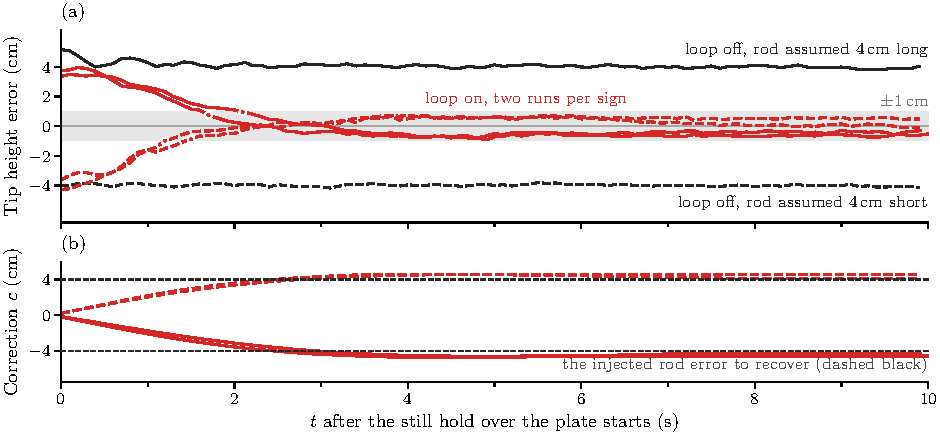
\includegraphics[width=\textwidth]{Images/tip_feedback.pdf}
\caption[Steering the measured magnet tip]{Steering the measured magnet tip in the rig twin (dry approach to the
plate, this work's own approach, twin only). The approach flies the UAV's body to the target plus an assumed rod
length; with that length 4\,cm wrong either way (solid: assumed long, dashed: assumed short) the measured tip parks
4\,cm high or low with the loop off (black). With the measured-tip loop on (red, two runs per sign) a slow, bounded
correction of the body goal brings the tip within 1\,cm of its setpoint (shaded) 1.2--2.1\,s after the still hold over
the plate begins (dots). (a) Tip height error: the measured tip height minus its setpoint. (b) The correction $c$ added
to the body goal; dashed black: the injected rod error. The loop integrates only in the still hold and freezes inside a
5\,mm deadband, on a contact and on an invalid tip.}
\label{fig:tip_feedback}
\end{figure}

\subsection{Dated history}
\label{sec:app_history}

Results flown on earlier code or earlier plants, superseded by the results above and kept one line each so that they
are not repeated.
\begin{itemize}
    \item \textbf{Trajectories, 4--5 October} (integral off, the earlier stack): three and four UAVs on hover, line,
    circle, figure-eight and spin, mean error 0.5--0.9\,cm; replaced by the carry claim (Table~\ref{tab:T7t}).
    \item \textbf{The resize in hover, 4--5 October}: peak 2.8--4.0$^\circ$, back in band in 0.9--1.0\,s on an
    announced detach; replaced by the unannounced release on the freeze tree (Figure~\ref{fig:detach}).
    \item \textbf{Landings, 4--5 October}: the unwind, ramp and idle tipped 0 of 18 against 2 of 21 straight descents;
    replaced by Table~\ref{tab:land}.
    \item \textbf{Layouts, 25 September} (earlier plant): after a release the even ring of four peaked at
    25.6--28.5$^\circ$ against 3.0--3.3$^\circ$ on plates 3, 7, 9 and 11; replaced by the support-margin curve
    (Figure~\ref{fig:F12}).
    \item \textbf{Hover, twin against the rig, 3 October}: holding the breakaway cap reproduced the rig's height
    shortfall (Section~\ref{sec:res_cap}).
    \item \textbf{The measured pull in the twin, 7 October} (exploratory): no abort or tip-over; superseded by the
    carry claim.
    \item \textbf{Command delay, 7 October} (exploratory): 0.05\,s or more of delay tipped UAVs at takeoff; the 15--45\,ms
    check of Section~\ref{sec:simulation} supersedes it.
    \item \textbf{The weld joint ladder, August} (earlier plant): a ball joint, a rod with inertia and a mid-span joint
    behaved alike, and a rigid weld capsized the ring in 5 of 5; compliance was not the cause of the weld transient.
    \item \textbf{The ground join, September} (earlier plant): the collaborator's controller joined four UAVs to the ring
    on the floor in two runs, then rocked it in four of the next five until the emulated rate loop used the gyro.
    \item \textbf{The rejoin mission, late September} (earlier plant): completed in two runs with a peak tilt at the
    rejoin of 1.6--1.7$^\circ$; in the rig twin before the co-motion confirmation the full mission reattached in hover
    in 2 of 2 runs and on the circle in 7 of 11 across code trees.
    \item \textbf{The join claim on the contact-and-lift proof, 12 October}: in hover the twin admitted the newcomer in
    5 of 5 runs with a ring tilt of 1.8--2.4$^\circ$; superseded by the co-motion confirmation of 14 October
    (Section~\ref{sec:res_join}).
\end{itemize}

\section{Development timeline}
\label{sec:app_timeline}

\begin{table}[H]
\centering
\small
\caption{Main steps of the work, 2026.}
\label{tab:app_timeline}
\begin{tabularx}{\textwidth}{lX}
\toprule
When & Step \\
\midrule
Feb--Apr & ROS~2 and Gazebo environment; four-UAV formation flight in simulation; one UAV with a tethered load \\
Jun & Cable models (spring--damper, then rigid rods); first port of the load--cable planner \\
Jul & Three UAVs carrying a payload with rigid rods in simulation; first rig flights; the network controller and the first mid-flight detach \\
Aug & Experiment runner; OCP resize against the network's hand-off; attach integration and the weld-joint ladder \\
early Sep & Runtime attachment geometry and detach by OCP resize; layout studies \\
mid Sep & The 0.86\,kg ring in every model; measured rod lengths; rod sweep from the floor; height integral; first carry attempts on the rig \\
late Sep & Attach by OCP resize; integration with the collaborator's controllers; rig days with the first lifts and the thrust identification; the rig twin \\
1--4 Oct & Three-UAV rig flights to 1.0\,m; the breakaway cap and its release; the tracker initial-condition fix; integral action in the planner's model \\
5--8 Oct & The rig twin becomes the simulation; the measured rod pull and rods planned at 60$^\circ$; four-UAV carries and releases on the rig; drop and land \\
9--12 Oct & The freed UAV disarmed alone; LAND in every phase; the newcomer's fall-backs; the release metrics, the resolution rule and the ledger bands frozen \\
14--15 Oct & The first attach flights on the rig; the co-motion confirmation; the drop rule in every mode \\
16--17 Oct & Freeze batches: the carry envelope, the levers on a release, drop and land, the re-flown appendix tables; the touchdown re-arm \\
\bottomrule
\end{tabularx}
\end{table}

\section{The network controller on the earlier plant}
\label{sec:app_network}

Everything in this appendix was flown on the earlier simulation plant (the 0.6\,kg disc and then the 0.86\,kg ring on
0.5\,m rods, 0.64\,kg UAVs and a linear thrust map), before the rig twin existed; none of it is re-flown, and the main
text does not rest on it. It answers the project plan's secondary question, whether a decentralised network controller
or the trajectory-based planner better balances robustness and tracking, and is kept as dated history.

The second reference generator was a port of the decentralised passivity-based controller of Quan et al.\
\cite{quan2025swarm} to rigid rods, the ring and the same trackers. Each UAV was a node of a virtual spring--damper
network, joined to a payload node at the desired payload position, to an anchor above it and to its neighbours, and
damped relative to all of them; the node's position, carried out one rod length from the UAV's own attachment point,
was the UAV's reference. A member leaving or joining is the network's native mode: it needs no new solver and no
redistribution designed by hand. Table~\ref{tab:detach_ab} gives the comparison that decided the question. Tracking:
with the network flying a circle the payload traced a circle 18\,\% too small and 0.68\,s late, most of it lost in a
stiff position tracker that the network's own architecture does not have; a velocity loop in its place restored the
radius at the cost of more tilt after the manoeuvre (5.4 against 1.4$^\circ$). Reconfiguration: Table~\ref{tab:detach_ab}.
The reasons the planner was kept are three: with rigid rods the payload is held by geometry, which the network can only
approximate; its damping acts on virtual nodes rather than on the payload; and it could not use the measured payload
pose without destabilising itself.

\begin{table}[h]
\centering
\small
\caption{The planner's OCP resize against the network on the earlier plant (Gazebo and the software-in-the-loop
bench).}
\label{tab:detach_ab}
\begin{tabularx}{\textwidth}{>{\raggedright\arraybackslash}Xcc}
\toprule
 & OCP resize & Network \\
\midrule
Detach, 4 to 3 on a circle, 0.4\,kg payload: settled payload tilt & about 1$^\circ$ & 26--48$^\circ$ \\
\quad survivors' tracking error & about 1\,mm & 60--910\,mm \\
Detach, 0.86\,kg ring, bench & survivors level within 0.5--2$^\circ$ & aborted at 53--61$^\circ$ \\
Attach, 0.86\,kg ring, bench & weld peak about 10$^\circ$ & capsized within about 8\,s of every weld \\
\bottomrule
\end{tabularx}
\end{table}
